\documentclass[a4paper,12pt,russian]{extarticle}
\usepackage[T2A,TS1]{fontenc}
\usepackage[russian]{babel}
\usepackage[lmargin=25mm,rmargin=25mm,tmargin=25mm,bmargin=30mm]{geometry}
\usepackage[onehalfspacing]{setspace}
\RequirePackage{caption}
\usepackage{graphicx}








%\newcommand{\T}[2]{T^{\left( #1 , #2 \right)} }
\newcommand{\ga}[1]{\Gamma^{\left( #1 \right)} }
\renewcommand{\P}[2]{\Pr\left( #1 \left| #2\right.\right)}

%\newcommand*{\hm}[1]{#1\nobreak\discretionary{}%
%{\hbox{$\mathsurround=0pt #1$}}{}}

\newcommand{\Mark}{\{(\Gamma_i, \varkappa_i); i \geqslant 0\}}
\newcommand{\MarkThree}{\{(\Gamma_i, \varkappa_{3,i}); i \geqslant 0\}}
\makeatletter
\newcommand{\rmnum}[1]{\romannumeral #1}
\newcommand{\Rmnum}[1]{\expandafter\@slowromancap\romannumeral #1@}
\makeatother
\newcommand{\No}{\textnumero}
\newcommand{\ml}[1]{\begin{multline}#1\end{multline}}
\newcommand{\mll}[1]{\begin{multline*}#1\end{multline*}}

\usepackage[Magistr]{../MyPackages/ptvstyle}
%\selectlanguage{russian}
\title{Моделирование и анализ системы обслуживания конфликтных потоков в классе приоритетных алгоритмов}
\author{студент группы 85М1\\ Кочеганов В.~М.}
\advisor{к.ф.-м.н., доцент \\ Зорин А.~В.}
\chief{д.ф.-м.н., профессор \\ Федоткин М.~А.}
\date{2014}


\begin{document}
\numberwithin{equation}{section}
\section{Постановка задачи и построение математической модели}

\subsection{Постановка задачи на содержательном уровне}

Рассмотрим систему массового обслуживания следующего вида (Рис.~\ref{SystemScheme}).
\begin{figure}[h]
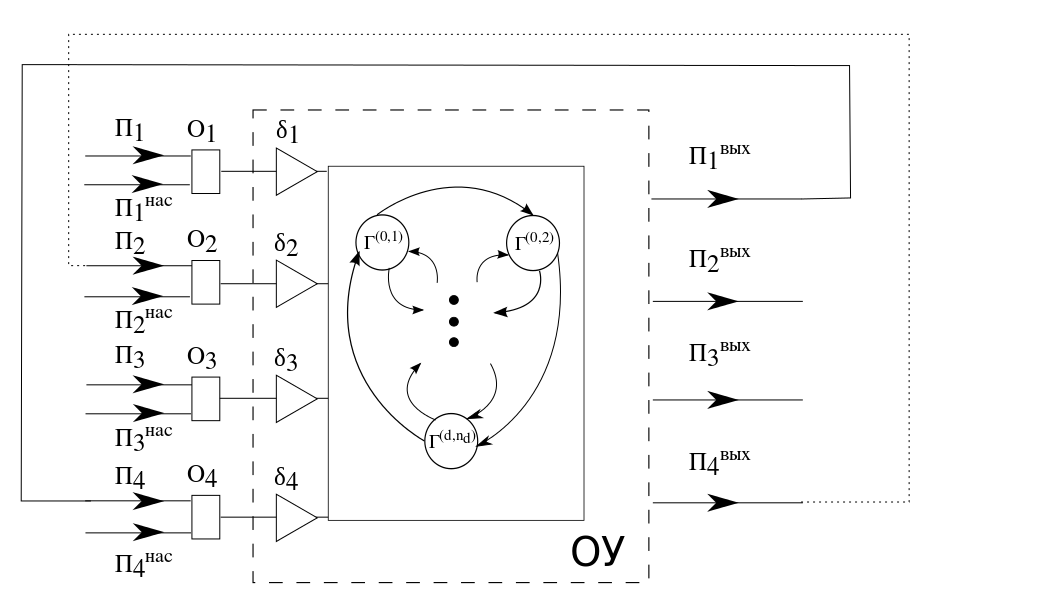
\includegraphics[scale=0.5]{SystemScheme.png} 
\caption{Структурная схема системы обслуживания}
\label{SystemScheme}
\end{figure}

Пусть в систему с одним обслуживающим устройством поступают потоки $\Pi_1$, $\Pi_2$, $\Pi_3$  и $\Pi_4$. Требования по потоку $\Pi_j$ становятся в соответствующую очередь $O_j$ с неограниченной вместимостью, $j\in \{1, 2, 3, 4\}$. Для $j \in \{1, 2, 3\}$ дисциплина очереди $O_j$, поддерживаемая устройством $\delta_j$, имеет тип FIFO (First In First Out). Таким образом, для обслуживания из соответствующей очереди выбирается то требование, которое пришло раньше. Дисциплина очереди $O_4$ будет описана ниже. Входные потоки $\Pi_1$ и $\Pi_3$ формируются внешней средой, которая, будем предполагать, имеет только одно состояние, то есть вероятностная структура потоков не меняется с течением времени. Требования потоков $\Pi_1$ и $\Pi_3$ формируют независимые между собой неординарные пуассоновские потоки, то есть  стационарные, без последействия и ординарные потоки групп требований. Интенсивности соответствующих простейших потоков для $\Pi_1$ и $\Pi_3$ будем обозначать $\lambda_1$ и $\lambda_3$, а распределение числа заявок в группе по потоку $\Pi_j$ будем описывать производящей функцией
$$
f_j(z) = \sum_{\nu=1}^{\infty} p_{\nu}^{(j)} z ^{\nu}, \quad j\in \{1,3\}, \eqno{(1)}
$$
\begin{equation}
f_j(z) = \sum_{\nu=1}^{\infty} p_{\nu}^{(j)} z ^{\nu}, \quad j\in \{1,3\},
\label{GeneratingFunc}
\end{equation}
которая предполагается аналитической при любом $z\in \mathbb{C}$ таком, что $|z|<(1+\varepsilon)$, $\varepsilon>0$. Величина $p_{\nu}^{(j)}$ определяет вероятность того, что по потоку $\Pi_j$ число требований в группе равно $\nu$. Обслуженные требования потока $\Pi_1$ поступают на повторное обслуживание, формируя при этом поток $\Pi_4$. Потоки $\Pi_2$ и $\Pi_3$ являются конфликтными, что означает запрет на одновременное обслуживание требований этих потоков и, следовательно, исследование системы не может быть сведено к задаче с меньшим числом потоков. 
 
 В каждый момент времени обслуживающее устройство находится в одном из конечного множества состояний $\Gamma=\{\Gamma^{(k,r)} \colon k=0,1,\ldots,d; r=1,2,\ldots n_k\}$ с заданными натуральными числами $d$, $n_0$, $n_1$, $\ldots$, $n_d$. В каждом состоянии $\ga{k,r}$ обслуживающее устройство находится в течение времени $T^{(k,r)}$. Введем множества $\Gamma^{\mathrm{I}}$, $\Gamma^{\mathrm{II}}$, $\Gamma^{\mathrm{III}}$ и $\Gamma^{\mathrm{IV}}$ следующим образом. В состоянии $\gamma \in \Gamma^{\mathrm{\Rmnum{1}}}$ обслуживаются только требования из очередей $O_1$, $O_2$ и $O_4$.
В состоянии $\gamma \in \Gamma^{\mathrm{\Rmnum{2}}}$ обслуживаются только требования из очередей $O_2$ и $O_4$.
В состоянии $\gamma \in \Gamma^{\mathrm{\Rmnum{3}}}$ обслуживаются только требования из очередей $O_1$, $O_3$ и $O_4$.
В состоянии $\gamma \in \Gamma^{\mathrm{\Rmnum{4}}}$ обслуживаются только требования из очередей $O_3$ и $O_4$.
Тогда множество $\Gamma$ есть объединение $\Gamma = \Gamma^{\mathrm{I}} \cup \Gamma^{\mathrm{II}} \cup \Gamma^{\mathrm{III}} \cup \Gamma^{\mathrm{III}}$ непересекающихся подмножеств. Также в дальнейшем нам понадобятся множества ${}^1\Gamma=\Gamma^{\mathrm{\Rmnum{1}}} \cup \Gamma^{\mathrm{\Rmnum{3}}}$, 
${}^2\Gamma=\Gamma^{\mathrm{\Rmnum{1}}} \cup \Gamma^{\mathrm{\Rmnum{2}}}$,
${}^3\Gamma=\Gamma^{\mathrm{\Rmnum{3}}} \cup \Gamma^{\mathrm{\Rmnum{4}}}$. 

Смена состояний обслуживающего устройства осуществляется по следующему правилу. Множество состояний $C_k = \{\Gamma^{(k,r)} \colon r=1,2,\ldots n_k\}$ будем называть $k$-м циклом, $k=1$, $2$, $\ldots$, $d$ (Рис. \ref{GraphScheme}). При $k=0$ состояние вида $\ga{0,r}$ будем называть состоянием продления, $r=0$, $1$, $\ldots$, $n_0$. Положим $r \oplus_k 1 = r+1$ для $r<n_k$ и $r \oplus_k 1 = 1$ при $r=n_k$, $k = 0$, $1$, $\ldots$, $d$. В цикле $C_k$ выделим подмножества $C_k^{\mathrm{O}}$ выходных, $C_k^{\mathrm{I}}$ входных и $C_k^{\mathrm{N}} = C_k \setminus (C_k^{\mathrm{O}} \cup C_k^{\mathrm{I}})$ нейтральных состояний. Тогда после состояния $\ga{k,r} \hm\in C_k\setminus C_k^{\mathrm{O}}$ обслуживающее устройство переходит в состояние $\ga{k,r \oplus_k 1}$ того же цикла $C_k$. При $\ga{k,r}$ принадлежащем множеству $C_k^{\mathrm{O}}$ прибор переходит в состояние $\ga{k,r\oplus_k 1}$, если число требований в очереди $O_3$ в момент переключения больше заданного порога $L$. В противном случае, то есть если число требований в очереди $O_3$ меньше либо равно $L$, то новое состояние прибора будет состоянием продления $\ga{0,r_1}$, где $r_1=h_1(\ga{k,r})$ и $h_1(\cdot)$~--- заданное отображение множества $\bigcup\limits_{k=1}^d C_k^{\mathrm{O}}$ во множество $\{1,2,\ldots, n_0\}$. После состояния $\ga{0,r}$ выбирается состояние того же вида $\ga{0,r_2}$, если число требований в очереди $O_3$ меньше или равно $L$, где $r_2=h_2(r)$ и $h_2(\cdot)$~--- заданное отображение множества $\{1,2, \ldots, n_0\}$ на себя; в противном случае включается входное состояние $\ga{k,r_3} \in C_k^{\mathrm{I}}$, где $\ga{k,r_3}=h_3(r)$ и $h_3(\cdot)$~--- заданное отображение множества $\{1,2, \ldots, n_0\}$ на множество  $\bigcup\limits_{k=1}^d C_k^{\mathrm{I}}$. Считается, что все состояния продления $\ga{0,r}$ принадлежат множеству ${}^2 \Gamma$, а также верны соотношения $C_k^\mathrm{O}\subset {}^2 \Gamma$ и $C_k^\mathrm{I}\subset {}^3 \Gamma$. Также будем предполагать, что из любого состояния продления существует ребро во входную вершину некоторого цикла, а все циклы, в свою очередь, имеют ровно одно входное и одно выходное состояние. И последним предположением является то, что все вершины продления образуют один цикл.

\begin{figure}[hb]\centering
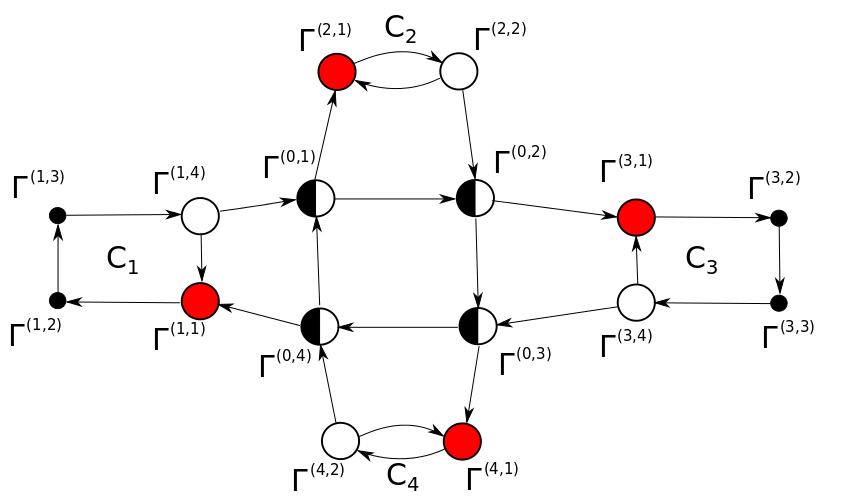
\includegraphics[scale=0.5]{GraphScheme3.png} 
\caption{Класс графов переходов. Незакрашенные вершины являются выходными вершинами, красным отмечены входные вершины, черным --- нейтральные, наполовину закрашенным вершинам соответствуют состояния продления}
\label{GraphScheme}
\end{figure}
%\subsection{Допустимые графы переходов состояний ОУ}

Таким образом, смена состояний обслуживающего устройства задается соотношением:
\begin{equation}
h(\ga{k,r},y) = 
\begin{cases}
\ga{k,r\oplus_k 1},& \quad \text{ если } \ga{k,r}\in C_k\setminus C_k^{\mathrm{O}};\\
\ga{k,r\oplus_k 1},& \quad \text{ если } \ga{k,r}\in C_k^{\mathrm{O}} \text{ и } y>L;\\
\ga{0,h_1(\ga{k,r})},& \quad \text{ если } \ga{k,r}\in C_k^{\mathrm{O}} \text{ и } y\leqslant L;\\
\ga{0,h_2(r)},& \quad \text{ если } k=0 \text{ и } y\leqslant L;\\
h_3(r),& \quad \text{ если } k=0 \text{ и } y > L.
\end{cases}
\label{hLaw}
\end{equation}

Рассмотрим введеные обозначения на примере рис.~\ref{GraphScheme}. Входными состояниями обслуживающего устройства 	являются $\ga{1,1} \in C_1^{\mathrm{I}}$, $\ga{2,1} \in C_2^{\mathrm{I}}$, $\ga{3,1} \in C_3^{\mathrm{I}}$ и $\ga{4,1} \in C_4^{\mathrm{I}}$, выходных состояний~--- $\ga{1,4} \in C_1^{\mathrm{O}}$, $\ga{2,2} \in C_2^{\mathrm{O}}$, $\ga{3,4} \in C_3^{\mathrm{O}}$ и $\ga{4,2} \in C_4^{\mathrm{O}}$, нейтральных состояний~--- $\ga{1,2}, \ga{1,3} \in C_1^{\mathrm{N}}$ и $\ga{3,2}, \ga{3,3} \in C_3^{\mathrm{N}}$. Состояния продления на графе представлены вершинами $\ga{0,1}$, $\ga{0,2}$, $\ga{0,3}$ и $\ga{0,4}$. Далее, отображение $h_1(\cdot)$ на графе задано таким образом, что оно переводит, например, выходное состояние $\ga{1,4}$ в число $1$~--- номер состояния продления $\ga{0,1}$, то есть $h_1(\ga{1,4})=1$. Аналогично, например, $h_2(1)=2$ и $h_2(3)=4$. Примером отображения $h_3(\cdot)$ является $h_3(2)=\ga{3,1}$.


Предполагается, что длительности обслуживания различных требований могут быть зависимыми и иметь различные законы распределения, поэтому вместо классического способа, состоящего в указании функции распределения длительности обслуживания произвольного требования, будут использованы потоки насыщения. Потоки насыщения $\Pi^{\mathrm{\text{нас}}}_j$, $j \in \{1,2,3,4\}$, определяются как виртуальные выходные потоки при 
условии максимального использования ресурсов обслуживающего устройства, а для $j\in \{1, 2, 3\}$ еще и при условии максимальной загрузки соответствующих очередей. Поток насыщения $\Pi^{\mathrm{\text{нас}}}_j$, $j\in \{1,2,3\}$, будет содержать неслучайное число $\ell_{k,r,j}$ требований, обслуженных в течение времени $T^{(k,r)}$, если $\ga{k,r} \in~^j\Gamma$, и будет содержать $0$ требований в противном случае: $\ga{k,r} \notin ~^j\Gamma$. Пусть $\mathbb{Z}_+$~--- множество целых неотрицательных чисел. Тогда, при условии, что в очереди $O_4$ находится $x \in \mathbb{Z}_+$ требований, поток насыщения $\Pi^{\mathrm{\text{нас}}}_4$ определим как поток, содержащий все $x$ требований.
%\subsection{Пример: тандем из двух перекрестков} 
Наконец, при состоянии обслуживающего устройства $\ga{k,r}$ каждое требование из очереди $O_4$ с вероятностью $p_{k,r}$ и независимо от других завершает обслуживание и отправляется в очередь $O_2$ потока~$\Pi_2$. С вероятностью $1-p_{k,r}$ требование очереди $O_4$ остается в ней до следующего такта. На следующем такте процесс повторяется.

В качестве наглядной физической интерпретации можно привести тандем из двух перекрестков (рис. \ref{crossroads}).
\begin{figure}[h]
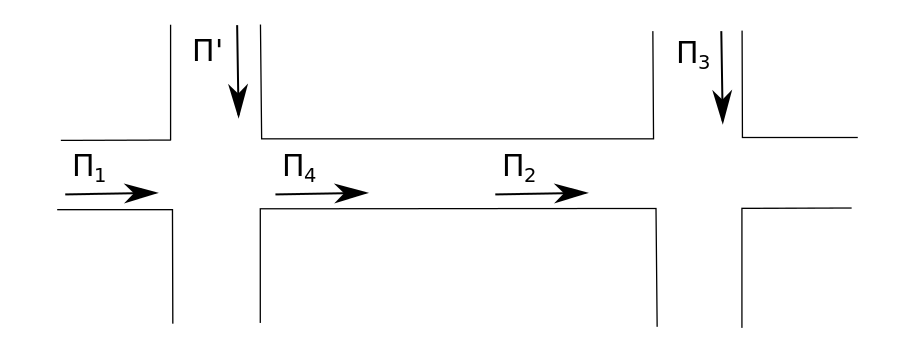
\includegraphics[scale=0.5]{Crossroads.png} 
\caption{Пример: тандем перекрестков}
\label{crossroads}
\end{figure}
В качестве потоков требований, формируемых внешней средой, выступают потоки прибывающих на перекрестки машин: конфликтные потоки $\Pi_1$, $\Pi_5$ на первом перекрестке, а также поток $\Pi_3$ на втором. Каждая машина из потока $\Pi_1$, проезжая первый перекресток, становится в очередь $O_4$ потока $\Pi_4$ и затем с некой вероятностью ($p_{k,r}$ для состояния $\ga{k,r}$ обслуживающего устройства) доезжает до следующего перекрестка, или же не успевает это сделать и остается в очереди $O_4$ до следующего такта обслуживания. В случае, если машина из очереди $O_4$ успевает доехать до второго перекрестка, она становится в очередь $O_2$ и ждет своей очереди для его прохождения.

Предполагается, что светофор на первом перекрестке имеет лишь два состояния $\{g_{1,1},g_{1,2}\}$: в состоянии $g_{1,1}$ машины потока $\Pi_1$ пропускаются фиксированное количество времени $\widetilde T^{(1,1)}$ (<<зеленый>> свет для $\Pi_1$); в состоянии $g_{1,2}$ --- простаивают в течение времени $\widetilde T^{(1,2)}$ (<<красный>> свет для $\Pi_1$). Светофор на втором перекрестке обслуживает по алгоритму с продлением: дополнительно к состоянию обслуживания потока $\Pi_3$ (состояние $g_{2,1}$), также имеется два состояния обслуживания потока $\Pi_2$ (состояния $\{g_{2,2},g_{2,3}\}$). Первое из них включается всегда после завершения обслуживания потока $\Pi_3$, а второе включается, если после очередного такта обслуживания потока $\Pi_2$ длина очереди $O_3$ не превосходит уровня $L$.
Длительности пребывания светофора на втором перекрестке в каждом из состояний суть $\widetilde T^{(2,1)}$, $\widetilde T^{(2,2)}$ и $\widetilde T^{(2,3)}$.


Рассматривая тандем из двух перекрестков как единую систему массового обслуживания и предполагая наблюдение за ней только в (дискретные) моменты переключения состояния хотя бы одного из светофоров, может быть показано, что количество различных состояний у полученной системы конечно. Действительно, положим, например, за состояние объединенной системы вектор $(g^{(1)},g^{(2)}, s, t)$, где $g^{(1)}\in \{g_{1,1},g_{1,2}\}$~--- состояние $1$--го перекрестка, $g^{(2)}\in \{g_{2,1},g_{2,2},g_{2,3}\}$~--- состояние $2$--го перекрестка, $s \in \{0, 1, 2\}$~--- номер последнего сменившего состояние перекрестка (принимает значение $0$ в случае, если сменили состояние оба перекрестка) и $t \in \{0, 1, 2, \ldots, T\}$~--- количество времени, оставшееся у продолжающего обслуживание с прошлого такта перекрестка (принимает значение $0$, если принимает значение $0$ величина $s$). Здесь $T$~--- максимальная длительность нахождения каждого из светофоров в одном состоянии. Тогда количество различных состояний не трудно посчитать и оно не будет превышать величины  $2\times 3 \times 3 \times T$.

В завершение построения примера отметим, что при прохождении перекрестков машины предполагаются движущимися только в прямом направлении, то есть перемешивания конфликтных потоков не допускается. Таким образом, поток $\Pi_5$ не представляет интереса для дальнейшего исследования системы и может быть отброшен и, следовательно, построенный пример целиком удовлетворяет структурной схеме на рис. \ref{SystemScheme}.

Теперь продемонстрируем на конкретном числовом примере выделение циклов и состояний продления. Пусть изменение состояний перекрестков и время пребывания (в секундах для определнности) в каждом из состояний задается графами на рис. \ref{SystemStates}.
\begin{figure}[h]
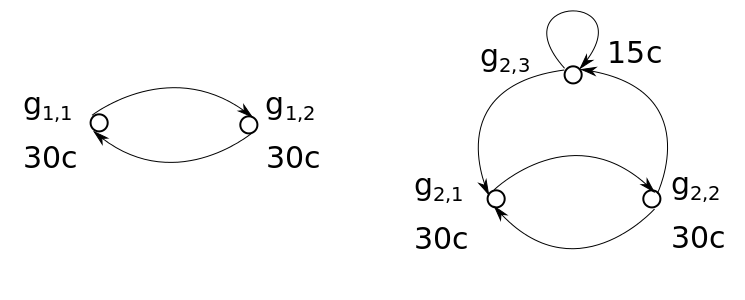
\includegraphics[scale=0.5]{SystemStates.png} 
\caption{Числовой пример тандема перекрестков. Левый граф соответствует первому перекрестку, правый~--- второму}
\label{SystemStates}
\end{figure}
За начальное состояние объединенной системы примем $\Gamma_0=(g_{1,1},g_{2,1},0,0)$, то есть первый перекресток находится в состоянии $g_{1,1}$, второй~--- в состоянии $g_{2,1}$, и оба только начали свою работу в своем состоянии (этот факт моделируется равенствами $s=0$ и $t=0$). Следующая смена состояний случится у обоих перекрестков одновременно и приведет к следующему состоянию $(g_{1,2},g_{2,2}, 0, 0)$. Далее смена состояний произойдет также у первого и второго перекрестков, однако второй перекресток может перейти как в состояние $g_{2,1}$, так и в состояние продления $g_{2,3}$. Таким образом следущим состоянием тандема будет либо опять $(g_{1,1},g_{2,1},0,0)$, либо $(g_{1,1},g_{2,3},0,0)$. Продолжая рассуждения аналогичным образом, получим следущий список всех возможных состояний системы:
\begin{align*}
(g_{1,1},g_{2,1},0,0)&=\ga{1,1} ,& \quad (g_{1,2},g_{2,2},0,0)&=\ga{1,2} ,& \quad (g_{1,1},g_{2,3},0,0)&=\ga{0,1}, \\
(g_{1,1},g_{2,3},15,2)&=\ga{0,2} ,& \quad (g_{1,2},g_{2,3},0,0)&=\ga{0,3} ,& \quad (g_{1,2},g_{2,3},15,2)&=\ga{0,4}, \\
(g_{1,2},g_{2,1},15,2)&=\ga{4,1} ,& \quad (g_{1,1},g_{2,1},15,1)&=\ga{4,2} ,& \quad (g_{1,1},g_{2,2},15,2)&=\ga{4,3}, \\
(g_{1,2},g_{2,2},15,1)&=\ga{4,4} ,& \quad (g_{1,2},g_{2,3},15,2)&=\ga{0,5} ,& \quad (g_{1,2},g_{2,1},0,0)&=\ga{3,1}, \\
(g_{1,1},g_{2,2},0,0)&=\ga{3,2} ,& \quad (g_{1,1},g_{2,1},15,2)&=\ga{2,1} ,& \quad (g_{1,2},g_{2,1},15,1)&=\ga{2,2}, \\
(g_{1,2},g_{2,2},15,2)&=\ga{2,3} ,& \quad (g_{1,1},g_{2,2},15,1)&=\ga{2,4}. & &
\end{align*}
В соответсвии с приведенными выше обозначениями, множества $C_1$, $C_2$, $C_3$, $C_4$, а также множество состояний продления строятся однозначным образом. Множествами входных состояний будут $C_1^{\mathrm{I}}=\{\ga{1,1}\}$, $C_2^{\mathrm{I}}=\{\ga{2,1}\}$, $C_3^{\mathrm{I}}=\{\ga{3,1}\}$ и $C_4^{\mathrm{I}}=\{\ga{4,1}\}$. Множествами выходных состояний будут $C_1^{\mathrm{O}}=\{\ga{1,2}\}$, $C_2^{\mathrm{O}}=\{\ga{2,4}\}$, $C_3^{\mathrm{O}}=\{\ga{3,2}\}$ и $C_4^{\mathrm{O}}=\{\ga{4,4}\}$. Функции $h_1(\cdot)$, $h_2(\cdot)$ и $h_3(\cdot)$ задаются поточечно:
\begin{equation*}
h_1(\ga{1,2})=1, \quad h_1(\ga{2,4})=2, \quad h_1(\ga{3,2})=3, \quad h_1(\ga{4,4})=5,
\end{equation*}
\begin{equation*}
h_2(1)=2, \quad h_2(2)=3, \quad h_2(3)=4 \quad h_2(4)=1, \quad h_2(5)=1,
\end{equation*}
\begin{equation*}
h_3(1)=\ga{2,1}, \quad h_3(2)=\ga{3,1}, \quad h_3(3)=\ga{4,1} \quad h_3(4)=\ga{1,1}, \quad h_3(5)=\ga{1,1}.
\end{equation*}
Этим завершается построение числового примера.

\subsection{Представление рассматриваемой системы обслуживания в виде кибернетической управляющей системы}
Описанная в предыдущем разделе на содержательном уровне система массового обслуживания должна рассматриваться как кибернетическая управляющая система обслуживания (см. \cite{Zorine:2011}). Схема управляющей системы приведена на рис. \ref{SystemScheme}. На схеме присутствуют следующие блоки: 1) внешняя среда с одним состоянием; 2) входные полюса первого типа~--- входные потоки $\Pi_1$, $\Pi_2$, $\Pi_3$, $\Pi_4$; 3) входные полюса второго типа~--- потоки насыщения $\Pi_1^{\mathrm{\text{нас}}}$, $\Pi_2^{\mathrm{\text{нас}}}$, $\Pi_3^{\mathrm{\text{нас}}}$, $\Pi_4^{\mathrm{\text{нас}}}$; 4) внешняя память~--- очереди $O_1$, $O_2$, $O_3$, $O_4$; 5) устройство по переработкe информации внешней памяти~--- устройства по поддержанию дисциплины очереди $\delta_1$, $\delta_2$, $\delta_3$, $\delta_4$; 6) внутренняя память~--- обслуживающее устройство (ОУ); 7) устройство по переработке информации во внутренней памяти~--- граф смены состояний; 8) выходные полюса $\Pi_1^{\mathrm{\text{вых}}}$, $\Pi_2^{\mathrm{\text{вых}}}$, $\Pi_3^{\mathrm{\text{вых}}}$, $\Pi_4^{\mathrm{\text{вых}}}$. Координатой блока является номер этого блока на схеме. 

Для задания информации блоков введем следующие величины и элементы, а также укажем множества их возможных значений. В качестве дискретной временной шкалы выберем последовательность $\tau_0=0$, $\tau_1$, $\tau_2$, $\ldots$ моментов смены состояний обслуживающего устройства. Обозначим $\Gamma_i$ из множества $\Gamma$ состояние обслуживающего устройства в течение времени $\left(\tau_{i-1};\tau_i\right]$, количество $\varkappa_{j,i} \in \mathbb{Z}_+ $ требований в очереди $O_j$ в момент времени $\tau_i$, количество $\eta_{j,i} \in \mathbb{Z}_+$ требований, поступивших в очередь $O_j$ по потоку $\Pi_j$ в течение времени $\left(\tau_{i};\tau_{i+1}\right]$, количество $\xi_{j,i} \in \mathbb{Z}_+$ требований по потоку насыщения $\Pi^{\mathrm{\text{нас}}}_j$ в течение времени $\left(\tau_{i};\tau_{i+1}\right]$, количество $\overline{\xi}_{j,i}\in \mathbb{Z}_+$ реально обслуженных требований по потоку $\Pi_j$ в течение времени $\left(\tau_{i};\tau_{i+1}\right]$, $j\in \{1,2,3,4\}$.

Закон изменения состояния обслуживающего устройства будем предполагать заданным соотношением 
\begin{equation}
\Gamma_{i+1}=h(\Gamma_i,\varkappa_{3,i}),
\label{gammaFunc}
\end{equation}
где отображение $h(\cdot,\cdot)$ определено в \eqref{hLaw}.
Для определения длительности $T_{i+1}$ состояния обслуживающего устройства в течение времени $\left(\tau_{i};\tau_{i+1}\right]$ удобно ввести функцию $h_T(\cdot,\cdot)$:
\begin{equation*}
T_{i+1}=h_T(\Gamma_i,\varkappa_{3,i})= T^{(k,r)},\quad  \text{ где } \ga{k,r}=\Gamma_{i+1}=h(\Gamma_i,\varkappa_{3,i}).
%\label{timeLaw}
\end{equation*}
Функциональная зависимость
\begin{equation}
\overline{\xi}_{j,i}=\min\{\varkappa_{j,i}+\eta_{j,i},\xi_{j,i}\}, \quad j\in \{1,2,3\},
\label{saturationEq}
\end{equation}
между величиной $\overline{\xi}_{j,i}$ и величинами $\varkappa_{j,i}$, $\eta_{j,i}$, $\xi_{j,i}$ реализует стратегию механизма обслуживания требований. Далее, поскольку 
\begin{equation*}
\varkappa_{j,i+1}=\varkappa_{j,i}+\eta_{j,i}-\overline{\xi}_{j,i}, \quad  j\in \{1,2,3\},
\end{equation*}
то из \eqref{saturationEq} следует соотношение
\begin{equation}
\varkappa_{j,i+1}=\max\{{0,\varkappa_{j,i}+\eta_{j,i}-\xi_{j,i}}\}, \quad j\in \{1,2,3\}.
\label{queuesFunc}
\end{equation}
Из формулировки поставленной задачи (см. также структурную схему на рис.~\ref{SystemScheme}) следуют соотношения для потока $\Pi_4$:
\begin{equation}
\eta_{4,i} = \min\{\xi_{1,i}, \varkappa_{1,i}+\eta_{1,i}\}, \quad \varkappa_{4,i+1}=\varkappa_{4,i}+\eta_{4,i}-\eta_{2,i}, \quad \xi_{4,i} = \varkappa_{4,i}.
\label{FourthFunc}
\end{equation}

Нелокальное описание входных потоков и потоков насыщения состоит в указании некоторых свойств условных распределений выделенных дискретных компонент $\eta_i=(\eta_{1,i},\eta_{2,i}, \eta_{3,i}, \eta_{4,i})$ и $\xi_i=(\xi_{1,i}, \xi_{2,i}, \xi_{3,i}, \xi_{4,i})$ маркированных точечных процессов \linebreak $\{(\tau_i, \nu_i, \eta_i); i\geqslant 0\}$ и $\{(\tau_i, \nu_i, \xi_i); i\geqslant 0\}$ при фиксированных значениях метки $\nu_i = (\Gamma_i;\varkappa_i)$, где $\varkappa_i=(\varkappa_{1,i},\varkappa_{2,i},\varkappa_{3,i},\varkappa_{4,i})$. 
Введем функции $\varphi_1(\cdot,\cdot)$ и $\varphi_3(\cdot,\cdot)$ из разложений 
\begin{equation*}
\sum_{\nu=0}^{\infty} z^\nu\varphi_j(\nu,t) = \exp\{\lambda_j t (f_j(z)-1)\},
\end{equation*}
где $f_j(z)$ определены в \eqref{GeneratingFunc}, $j \in \{1,3\}$. Функция $\varphi_j(\nu,t)$ есть вероятность поступления $\nu=0$, $1$, $\ldots$ требований по потоку $\Pi_j$ за время $t \geqslant 0$. Положим $\varphi_j(\nu,t)$ равной нулю при $\nu < 0$. Функцию $\psi(\cdot,\cdot,\cdot)$ зададим формулой
\begin{equation*}
\psi(k;y,u)=C_y^k u^k (1-u)^{y-k}.	
\end{equation*}
По своему смыслу $\psi(k;y,u)$ есть вероятность поступления $k$ требований по потоку $\Pi_2$ при условии, что очередь $O_4$ содержит $y$ требований и обслуживающее устройство находится в состоянии $\ga{k,r}$, так что $u=p_{k,r}$. При нарушении условия $ 0\leqslant k \leqslant y$ положим $\psi(k;y,u)$ равной нулю.

Пусть $a=(a_1, a_2, a_3, a_4) \in \mathbb{Z}_+^4$ и $x=(x_1, x_2, x_3, x_4) \in \mathbb{Z}_+^4$. Тогда из постановки задачи на содержательном уровне следует, что при фиксированном значении метки $\nu_i=(\ga{k,r}; x)$ вероятность $\varphi(a,k,r,x)$ одновременного выполнения равенств $\eta_{1,i}=a_1$, $\eta_{2,i}=a_2$, $\eta_{3,i}=a_3$, $\eta_{4,i}=a_4$ есть 
\begin{equation}
\varphi_1(a_1,h_T(\ga{{k},{r}},x_3)) \times \psi(a_2,x_4, p_{\tilde{k},\tilde{r}}) \times \varphi_3(a_3,h_T(\ga{{k},{r}},x_3))
\times \delta_{a_4,\min{\{\ell(\tilde{k},\tilde{r},1), x_1+a_1}\}},
\label{conditionProbOne}
\end{equation}
где $\ga{\tilde{k},\tilde{r}}=h(\ga{k,r},x_3)$ и $\delta_{i,j}$ есть символ Кронекера
\begin{equation*}
\delta_{i,j}=\begin{cases} 1, \quad \text{ если }i=j\\0, \quad \text{ если } i\neq j,
\end{cases}.
\end{equation*}
Пусть $b=(b_1, b_2, b_3, b_4) \in \mathbb{Z}_+^4$. Из содержательной постановки задачи также следует, что вероятность $\zeta(b, k, r, x)$ одновременного выполнения равенств $\xi_{1,i}=b_1$, $\xi_{2,i}=b_2$, $\xi_{3,i}=b_3$, $\xi_{4,i}=b_4$ при фиксированном значении метки $\nu_i=(\ga{k,r}; x)$ есть
\begin{equation}
\delta_{b_1,\ell(\tilde{k},\tilde{r},1)} \times \delta_{b_2,\ell(\tilde{k},\tilde{r},2)} \times 
\delta_{b_3,\ell(\tilde{k},\tilde{r},3)} \times \delta_{b_4,x_4}.
\label{conditionProbTwo}
\end{equation}
Из формулы \eqref{conditionProbTwo} следует для $j\in \{1, 2, 3\}$, что вероятность события $\xi_{j,i}=0$ равна $1$ в случае $h(\ga{k,r},x_3)\notin {}^j\Gamma$ и что вероятность события $\xi_{j,i}=\ell_{\tilde{k},\tilde{r},j}$ равна $1$, если $\ga{\tilde{k},\tilde{r}}=h(\ga{k,r},x_3)\in {}^j\Gamma$.


Содержательный смысл следующей теоремы состоит в том, что сформулированные выше функциональные связи и вероятностные свойства введенных объектов непротиворечивы и могут быть реализованы на некотором общем вероятностном пространстве.
%Построим теперь 	вероятностное пространство $(\Omega, {\cal F}, \Pr(\cdot))$, чтобы можно было рассматривать введеные величины как случайные величины на этом пространстве. А именно, докажем следующую теорему.
\begin{theorem}
Пусть $\gamma_0=\ga{k_0,r_0} \in \Gamma$ и $x^0=(x_{1,0},x_{2,0}, x_{3,0},x_{4,0})\in \mathbb{Z}_+^4$ фиксированы.
Тогда существует вероятностное пространство $(\Omega, {\cal F}, \Pr(\cdot))$ и заданные на нем случайные величины $\eta_{j,i}=\eta_{j,i}(\omega)$, $\xi_{j,i}=\xi_{j,i}(\omega)$, 	 $\varkappa_{j,i}=\varkappa_{j,i}(\omega)$ и случайные элементы $\Gamma_i=\Gamma_i(\omega)$, $i\geqslant 0$, $j\in \{1, 2, 3, 4\}$, такие, что 1) имеют место равенства $\Gamma_0(\omega) = \gamma_0$ и $\varkappa_0(\omega)=x^0$; 2) выполняются соотношения \eqref{gammaFunc}, \eqref{queuesFunc}, \eqref{FourthFunc}; 3) для любых  $a$, $b$, $x^t=(x_{1,t},x_{2,t},x_{3,t},x_{4,t}) \in \mathbb{Z}_+^4$, $\ga{k_t,r_t} \in \Gamma$, $t = 1, 2, \ldots$, условное распределение векторов $\eta_i$, и $\xi_i$ имеет вид
\begin{equation}
\Pr \left(\{ \omega \colon \eta_i = a, \xi_i=b\} \left|\bigcap_{t=0}^{i}\{\omega\colon \Gamma_t=\ga{k_t,r_t}, \varkappa_t=x^t\}\right.\right)=
\varphi(a,k_i,r_i,x^i)\times \zeta(b,k_i,r_i,x^i),
\label{ProbablititiesToProve}
\end{equation}
где функции $\varphi(\cdot, \cdot, \cdot, \cdot)$ и $\zeta(\cdot, \cdot, \cdot, \cdot)$ определяются формулами \eqref{conditionProbOne} и \eqref{conditionProbTwo} соответственно, $i \geqslant 0$.

\label{myTheorem}
\end{theorem}
\begin{proof}
В соответствии с теоремой Ионеску Тулчи (см. \cite{Shiryaev}) для доказательства достаточно задать на $(\Omega_0, {\cal F}_0)$ вероятностную меру $P_0(\cdot)$ и далее, считая для $0 < i \leqslant n$ и каждого набора элементарных исходов $(\omega_0, \omega_1, \ldots, \omega_{i-1})$ заданной на $(\Omega_i, {\cal F}_i)$ вероятностную меру $P(\omega_0,\omega_1,\ldots, \omega_{i-1};\cdot)$, задать на $(\Omega_{n+1}, {\cal F}_{n+1})$ меру $P(\omega_0,\omega_1,\ldots, \omega_{n};\cdot)$, причем для любого множества $B\in {\cal F}_i$ функции $P(\omega_0,\omega_1,\ldots, \omega_{i-1};B)$
должны быть измеримыми функциями от $(\omega_0, \omega_1, \ldots, \omega_{i-1})$. Тогда для декартова произведения пространств элементарных исходов $\Omega=\prod\limits_{i=0}^{\infty}\Omega_i$ и произведения $\sigma$-алгебр ${\cal F}=\bigotimes\limits_{i=0}^{\infty} {\cal F}_i$ на $(\Omega,{\cal F})$ будет существовать единственная вероятностная мера $\Pr(\cdot)$ такая, что для любого $i \geqslant 0$ верно равенство
\begin{equation}
\Pr\{\omega \colon \omega_0 \in A_0, \omega_1 \in A_1, \ldots, \omega_i\in A_i\} = P_i(A_0 \times A_1 \times \ldots \times A_i),
\label{ProbabilitiesGeneral}
\end{equation}
где 
\begin{equation}
 P_i(A_0 \times A_1 \times \ldots \times A_i) = \int_{A_0} P_0(d \omega_0) \int_{A_1} P(\omega_0;d \omega_1) \ldots \int_{A_i} P(\omega_0, \omega_1, \ldots, \omega_{i-1}; d \omega_i),
\label{ProbabilitiesGeneralOne}
\end{equation}
для любого $A_i$ из ${\cal F}_i$. 

Итак, за описание элементарного исхода $\omega_i \in \Omega_i$ для произвольного $i \geqslant 0$ примем набор $(\omega_{1,i},\omega_{2,i},\omega_{3,i})$, $\omega_{j,i}\in \mathbb{Z}_+$. Таким образом, $\Omega_i=\mathbb{Z}_+^3$ и в качестве $\sigma$-алгебры ${\cal F}_i$ возьмем множество всех подмножеств множества $\Omega_i$: ${\cal F}_i=2^{\Omega_i}$. Пусть $\ga{\tilde{k},\tilde{r}}=h(\ga{k_0,r_0},x_{3,0})$. Тогда  поскольку множество $\Omega_0$ счетно, определим вероятностную меру $P_0(\cdot)$ на измеримом пространстве $(\Omega_0,{\cal F}_0)$ ее значениями на одноточечных множествах:
\begin{equation}
P_0(\{(a_1,a_2,a_3)\})=\varphi_1(a_1,h_T(\ga{k_0,r_0})) \times \psi(a_2,x_{2,0}, p_{\tilde{k},\tilde{r}}) \times \varphi_3(a_3,h_T(\ga{k_0,r_0})).
\label{probabilitiesOne}
\end{equation}
Для $j\in \{1,2,3\}$ определим величины
\begin{equation}
\Gamma_0=\gamma_0, \quad \varkappa_{j,0}=x_{j,0}, \quad \xi_{j,0}=l(\tilde{k},\tilde{r},j), \quad \eta_{j,0}=\omega_{j,0},
\label{startRekOne}
\end{equation}
и
\begin{equation}
 \varkappa_{4,0}=x_{4,0}, \quad \xi_{4,0}=x_{4,0}, \quad \eta_{4,0}=\min\{\xi_{1,0}, x_{1,0}+\eta_{1,0}\}.
\label{startRekTwo}
\end{equation}

Теперь, предполагая заданными на $(\Omega_i, {\cal F}_i)$ вероятностные меры $P(\omega_0, \omega_1, \ldots, \omega_{i-1};\cdot)$, заданными величины $\Gamma_i$, $\varkappa_{j,i}$, $\xi_{j,i}$, $\eta_{j,i}$, $i\in \{0,1,\ldots,n\}$, $j\in \{1, 2, 3, 4\}$ и фиксируя набор $(\omega_0, \omega_1, \ldots, \omega_{n})$, определим на $(\Omega_{n+1}, {\cal F}_{n+1})$ меру $P(\omega_0, \omega_1, \ldots, \omega_n;\cdot)$. Положим для $j\in \{1, 2, 3\}$
\begin{equation}
\Gamma_{n+1}=\ga{k^*,r^*}=h(\Gamma_{n},\varkappa_{3,n}), \quad \varkappa_{j,n+1}=\max\{ 0,\varkappa_{j,n}+\eta_{j,n} -\xi_{j,n}\},
\label{NextRekOne}
\end{equation}
\begin{equation}
\varkappa_{4,n+1}=\varkappa_{4,n}+\eta_{4,n}-\eta_{2,n}, \quad \xi_{j,n+1}=l(k^*,r^*,j),
\label{NextRekTwo}
\end{equation}
\begin{equation}
\eta_{j,n+1}=\omega_{j,n+1}, \quad \eta_{4,n+1}=\min\{\xi_{1,n+1}, \varkappa_{1,n+1}+\eta_{1,n+1}\}, \quad \xi_{4,n+1}=\varkappa_{4,n+1}.
\label{NextRekThree}
\end{equation}
Тогда, по аналогии с построением вероятностной меры $P_0(\cdot)$, зададим меру $P(\omega_0,\omega_1,\ldots,\omega_n;\cdot)$ на одноточечных множествах $\{(a_1,a_2,a_3)\}$:
\ml
{
P(\omega_0,\omega_1,\ldots,\omega_n;\{(a_1,a_2,a_3)\}) = \\
= \varphi_1(a_1,h_T(\Gamma_n,x_{3,n})) \times \psi(a_2,x_{4,n}, p_{k^*,r^*}) \times \varphi_3(a_3,h_T(\Gamma_n,x_{3,n})).
\label{probabilitiesTwo}
}
Вероятностное пространство $(\Omega,{\cal F},\Pr(\cdot))$ построено. 

Теперь докажем, что введеные с помощью формул \eqref{startRekOne}~--~\eqref{NextRekThree} случайные элементы $\Gamma_i(\omega)$ и случайные величины $\varkappa_{j,i}(\omega)$, $\eta_{j,i}(\omega)$, $\xi_{j,i}(\omega)$, $i \geqslant 0$, $j \in \{1, 2, 3, 4\}$ удовлетворяют условиям теоремы. Из формулы \eqref{NextRekOne} следует, что случайные элементы $\Gamma_i$ удовлетворяют соотношению \eqref{gammaFunc}, а случайные величины $\varkappa_{j,i}$ для $j\in \{1, 2, 3\}$ удовлетворяют соотношению \eqref{queuesFunc}. Из формулы \eqref{NextRekTwo} заключаем, что $\varkappa_{4,i}$ удовлетворяет соотношению $\eqref{FourthFunc}$. Далее, из \eqref{startRekTwo} и \eqref{NextRekThree} следует справедливость соотношений \eqref{FourthFunc} для величин $\eta_{4,i}$ и $\xi_{4,i}$. 

Перейдем к доказательству равенства \eqref{ProbablititiesToProve}. Для этого найдем явное выражение для условной вероятности $\Pr (\{ \omega \colon \eta_i = a, \xi_i=b\} | \bigcap_{t=0}^{i}\{\omega\colon \Gamma_t=\ga{k_t,r_t}, \varkappa_t=x^t\})$. Пусть $\ga{\tilde{k}_i,\tilde{r}_i}=h(\ga{k_i,r_i},x^i)$. Распишем по определению условной вероятности:
\ml
{
\Pr \left(\left\{ \omega \colon \eta_i = a, \xi_i=b\right\}  \left| \bigcap_{t=0}^{i}\left\{\omega\colon \Gamma_t=\ga{k_t,r_t}, \varkappa_t=x^t\right\}\right.\right) = \\
=\Pr\left(\{ \omega \colon \eta_i = a, \xi_i=b \} \cap \bigcap_{t=0}^{i}\{\omega\colon \Gamma_t=\ga{k_t,r_t}, \varkappa_t=x^t\}\right) \Big/
\Pr\left( \bigcap_{t=0}^{i}\{\omega\colon \Gamma_t=\ga{k_t,r_t}, \varkappa_t=x^t\}\right).
\label{Construction:1}
}
Далее из \eqref{ProbabilitiesGeneral}, \eqref{ProbabilitiesGeneralOne} и того факта, что $\Gamma_i$ и $\varkappa_{i}$ не зависят от $\omega_i$ (этот факт следует из \eqref{startRekOne}~--~\eqref{NextRekTwo}), получим выражение для знаменателя последней дроби
\ml
{
\Pr\left( \bigcap_{t=0}^{i}\{\omega\colon \Gamma_t=\ga{k_t,r_t}, \varkappa_t=x^t\}\right)=\\
=\sum_{\substack{\omega_0, \omega_1,\ldots \omega_{i-1} \colon \\ \Gamma_t=\ga{k_t,r_t}, \varkappa_t=x^t, \forall 0\leqslant t \leqslant i-1}} P_0(\omega_0)\times P(\omega_0;\{\omega_1\})\times\ldots\times P(\omega_0,\omega_1,\ldots, \omega_{i-2};\{\omega_{i-1}\}).
\label{Construction:2}
}
Преобразуем множество $\{ \eta_i = a, \xi_i=b \} \cap \{\Gamma_i=\ga{k_i,r_i}, \varkappa_i=x^i\}$, учитывая соотношения \eqref{startRekOne}~--~\eqref{NextRekThree}:
\mll
{
\left\{ \eta_i = a, \xi_i=b \right\} \cap \left\{\Gamma_i=\ga{k_i,r_i}, \varkappa_i=x^i\right\} = \left\{\Gamma_i=\ga{k_i,r_i}, \varkappa_i=x^i\right\} \cap\\
\cap \left\{ \eta_{j,i} = a_j, j\in \{1, 2, 3\}\right\} \cap \left\{ \xi_{j,i} = b_j, j\in \{1, 2, 3\}\right\} \cap \left\{ \xi_{4,i} = b_4 \right\} \cap  \left\{ \eta_{4,i} = a_4 \right\} = \\
= \left\{\Gamma_i=\ga{k_i,r_i}, \varkappa_i=x^i\right\} \cap \left\{ \omega_{j,i} = a_j, j\in \{1, 2, 3\}\right\} \cap \left\{ b_j=\ell(\tilde{k}_i,\tilde{r}_i,j), j\in \{1, 2, 3\}\right\} \cap \\ 
\cap \left\{ b_4 = x_{4,i} \right\} \cap  \left\{ a_4=\min\left\{\ell(\tilde{k}_i,\tilde{r}_i,1), x_{1,i}+a_1\right\} \right\}. 
}
Тогда для числителя дроби из \eqref{Construction:1} имеем:
\ml
{
\Pr\left(\{ \omega \colon \eta_i = a, \xi_i=b \} \cap \bigcap_{t=0}^{i}\{\omega\colon \Gamma_t=\ga{k_t,r_t}, \varkappa_t=x^t\}\right)=\\
= \Pr\left(\left\{ \eta_i = a, \xi_i=b \right\} \cap \left\{\Gamma_i=\ga{k_i,r_i}, \varkappa_i=x^i\right\} \cap \bigcap_{t=0}^{i-1}\{\omega\colon \Gamma_t=\ga{k_t,r_t}, \varkappa_t=x^t\}\right)=\\
= \delta_{b_4,x_{4,i}} \times \delta_{a_4,\min\left\{\ell(\tilde{k}_i,\tilde{r}_i,1), x_{1,i}+a_1\right\}} \times \prod_{j=1}^3\delta_{b_j,\ell(\tilde{k}_i,\tilde{r}_i,j)}   \times \\
\times \Pr\left( \left\{ \omega_{j,i} = a_j, j\in \{1, 2, 3\}\right\} \cap \left\{\Gamma_i=\ga{k_i,r_i}, \varkappa_i=x^i\right\} \cap \bigcap_{t=0}^{i-1}\{\omega\colon \Gamma_t=\ga{k_t,r_t}, \varkappa_t=x^t\}\right)
\label{Construction:3}
}
И по аналогии со знаменателем (выражение \eqref{Construction:2}), распишем последнюю вероятность:
\mll
{
\Pr\left( \left\{ \omega_{j,i} = a_j, j\in \{1, 2, 3\}\right\} \cap \left\{\Gamma_i=\ga{k_i,r_i}, \varkappa_i=x^i\right\} \cap \bigcap_{t=0}^{i-1}\{\omega\colon \Gamma_t=\ga{k_t,r_t}, \varkappa_t=x^t\}\right) =\\
= \sum_{\substack{\omega_0, \omega_1,\ldots \omega_{i-1} \colon \\ \Gamma_t=\ga{k_t,r_t}, \varkappa_t=x^t, \forall 0\leqslant t \leqslant i-1}} P_0(\omega_0)\times P(\omega_0;\{\omega_1\})\times\ldots\times P(\omega_0,\omega_1,\ldots, \omega_{i-2};\{\omega_{i-1}\})\times\\
\times  P(\omega_0,\omega_1,\ldots, \omega_{i-1};\{(a_1, a_2, a_3)\}) =
}
и подставляя \eqref{probabilitiesTwo}, получим
\ml
{
=\varphi_1(a_1,h_T(\Gamma_i,x_{3,i})) \times \psi(a_2,x_{4,i}, p_{\tilde{k}_i,\tilde{r}_i}) \times \varphi_3(a_3,h_T(\Gamma_i,x_{3,i})) \times \\ 
\times \sum_{\substack{\omega_0, \omega_1,\ldots \omega_{i-1} \colon \\ \Gamma_t=\ga{k_t,r_t}, \varkappa_t=x^t, \forall 0\leqslant t \leqslant i-1}} P_0(\omega_0)\times P(\omega_0;\{\omega_1\})\times\ldots\times P(\omega_0,\omega_1,\ldots, \omega_{i-2};\{\omega_{i-1}\}).
\label{Construction:4}
}
Подставляя  \eqref{Construction:4} в \eqref{Construction:3}, а затем \eqref{Construction:3} и \eqref{Construction:2} в \eqref{Construction:1}, получим:
\mll
{
\Pr \left(\left\{ \omega \colon \eta_i = a, \xi_i=b\right\}  \left| \bigcap_{t=0}^{i}\left\{\omega\colon \Gamma_t=\ga{k_t,r_t}, \varkappa_t=x^t\right\}\right.\right)  = \\
= \delta_{b_4,x_{4,i}} \times \delta_{a_4,\min\left\{\ell(\tilde{k}_i,\tilde{r}_i,1), x_{1,i}+a_1\right\}} \times \prod_{j=1}^3\delta_{b_j,\ell(\tilde{k}_i,\tilde{r}_i,j)} \times
\varphi_1(a_1,h_T(\Gamma_i,x_{3,i})) \times \\ \times \psi(a_2,x_{4,i}, p_{\tilde{k}_i,\tilde{r}_i}) 
\times  \varphi_3(a_3,h_T(\Gamma_i,x_{3,i})) \times \\ 
\times \sum_{\substack{\omega_0, \omega_1,\ldots \omega_{i-1} \colon \\ \Gamma_t=\ga{k_t,r_t}, \varkappa_t=x^t, \forall 0\leqslant t \leqslant i-1}} P_0(\omega_0)\times P(\omega_0;\{\omega_1\})\times\ldots\times P(\omega_0,\omega_1,\ldots, \omega_{i-2};\{\omega_{i-1}\}) \Big/ \\
\Big/ \sum_{\substack{\omega_0, \omega_1,\ldots \omega_{i-1} \colon \\ \Gamma_t=\ga{k_t,r_t}, \varkappa_t=x^t, \forall 0\leqslant t \leqslant i-1}} P_0(\omega_0)\times P(\omega_0;\{\omega_1\})\times\ldots\times P(\omega_0,\omega_1,\ldots, \omega_{i-2};\{\omega_{i-1}\})
}
и после сокращения одинаковых сумм получаем в точности \eqref{ProbablititiesToProve}.
\end{proof}

\begin{corollary}
В условиях предыдущей теоремы верно равенство
\ml
{
\Pr \left(\{ \omega \colon \eta_i = a, \xi_i=b\} \left|\bigcap_{t=0}^{i}\{\omega\colon \Gamma_t=\ga{k_t,r_t}, \varkappa_t=x^t\}\right.\right)=\\
=\Pr \left(\{ \omega \colon \eta_i = a, \xi_i=b\} \left|\{\omega\colon \Gamma_i=\ga{k_i,r_i}, \varkappa_i=x^i\}\right.\right)
\label{eta:xi:forgetProperty}
}
%и
%\ml
%{
%\Pr \left(\{ \omega \colon \eta_{3,i} = a_3, \xi_{3,i}=b_3\} \left|\bigcap_{t=0}^{i}\{\omega\colon \Gamma_t=\ga{k_t,r_t}, \varkappa_t=x^t\}\right.\right)=\\
%=\Pr \left(\{ \omega \colon \eta_{3,i} = a_3, \xi_{3,i}=b_3\} \left|\bigcap_{t=0}^{i}\{\omega\colon \Gamma_t=\ga{k_t,r_t}, \varkappa_{3,t}=x_3^t\}\right.\right)=\\
%=\Pr \left(\{ \omega \colon \eta_{3,i} = a_3, \xi_{3,i}=b_3\} \left|\{\omega\colon \Gamma_i=\ga{k_i,r_i}, \varkappa_{3,i}=x_3^i\}\right.\right)
%\label{eta:xi:three:forgetProperty}
%}

\label{eta:xi:forget}
\end{corollary}
\begin{proof}
Действительно, из \eqref{ProbablititiesToProve} cледует, что вероятность, стоящая в левой части равенства \eqref{eta:xi:forgetProperty}, равна величине $\varphi(a,k_i,r_i,x^i)\times \zeta(b,k_i,r_i,x^i)$, зависящей только от значения $(\ga{k_i,r_i},x^i)$ пары $(\Gamma_i,\varkappa_i)$ и не зависящей от значений остальных пар $(\Gamma_t,\varkappa_t)_{0\leqslant t \leqslant i-1}$. Таким образом, знание о значениях пар $(\Gamma_t,\varkappa_t)_{0\leqslant t \leqslant i-1}$ не влияет на вероятность $\Pr (\{ \omega \colon \eta_i = a, \xi_i=b\} |\bigcap_{t=0}^{i}\{\omega\colon \Gamma_t=\ga{k_t,r_t}, \varkappa_t=x^t\})$ и, следовательно, \eqref{eta:xi:forgetProperty} верно.

%Аналогично, из \eqref{ProbablititiesToProve} можно заключить, что вероятность $\Pr (\{ \omega \colon \eta_{3,i} = a_3, \xi_{3,i}=b_3\} |\bigcap_{t=0}^{i}\{\omega\colon \Gamma_t=\ga{k_t,r_t}, \varkappa_t=x^t\})$ равна величине $\varphi_3(a_3,h_T(\ga{{k_i},{r_i}},x_3^i))\times \delta_{b_3,\ell(\tilde{k},\tilde{r},3)}$, $\ga{\tilde{k},\tilde{r}}=h(\ga{k_i,r_i},x_3^i)$, зависящей только от значений $(\ga{k_i,r_i},x_3^i)$ пары $(\Gamma_i,\varkappa_{3,i})$. Следовательно, равенства \eqref{eta:xi:three:forgetProperty} также верны.
\end{proof}

Введем для $y_0$, $y$, $\tilde{y} \in \mathbb{Z}_+$ и $t \in \mathbb{R}$, $t\geqslant 0$ функции
\begin{equation}
\begin{aligned}
\widetilde{\psi}(k,r,y_0,y,\tilde{y}) &= 
\begin{aligned}[t]
&(1 - \delta_{\tilde{y},0}) \psi(\tilde{y}+\ell(k,r,2)-y,y_0, p_{k,r})  +\\
&+ \delta_{\tilde{y},0}\sum_{a=0}^{\ell(k,r,2)-y} \psi(a,y_0, p_{k,r}),
\end{aligned}\\
\widetilde{\varphi}_3(k,r,t,y,\tilde{y}) &= (1-\delta_{\tilde{y},0}) \varphi_3(\tilde{y} + \ell(k,r,3)-y,t)  +\delta_{\tilde{y},0}\sum_{a=0}^{\ell(k,r,3)-y} \varphi_3(a,t).
%,\\
%\widetilde{\varphi}_{1}(k,r,t,x,\tilde{x},a) &=
%\begin{aligned}[t]
%& \varphi_1(\tilde{x}-x + \ell(k,r,1),t) (1 - \delta_{\tilde{x},0}) \delta_{a,\ell(k,r,1)} +\\
%&+\delta_{\tilde{x},0}\sum_{a_1=0}^{\ell(k,r,1)-x} \varphi_1(a_1,t) \times \delta_{a,x+a_1},
%\end{aligned}
\end{aligned}
\label{tildephi}
\end{equation}
причем $k$ и $r$ такие, что $\ga{k,r}\in \Gamma$.
	
\begin{corollary}
Пусть $\ga{k_{i+1},r_{i+1}}=h(\ga{k_i,r_i},x_{3,t})$. Тогда в условиях теоремы~\ref{myTheorem} верны равенства
\begin{align}
&\Pr (\{ \omega \colon \varkappa_{2,i+1} = x_{2,i+1}\} |\cap_{t=0}^{i}\{\omega\colon \Gamma_t=\ga{k_t,r_t}, \varkappa_t=x^t\})=\widetilde{\psi}(k_{i+1},r_{i+1},x_{4,i},x_{2,i},x_{2,i+1}),
\label{kappa:2:conditional}\\
&\Pr (\{ \omega \colon \varkappa_{3,i+1} = x_{3,i+1}\} |\cap_{t=0}^{i}\{\omega\colon \Gamma_t=\ga{k_t,r_t}, \varkappa_t=x^t\})=\widetilde{\varphi}_3(k_{i+1},r_{i+1},h_T(\ga{k_i,r_i},x_{3,i}),x_{3,i},x_{3,i+1}),
\label{kappa:3:conditional}
\end{align}
\end{corollary}
\begin{proof}
Начнем с доказательства равенства \eqref{kappa:2:conditional}. Распишем по формуле полной вероятности, а затем учтем \eqref{ProbablititiesToProve} и \eqref{eta:xi:forgetProperty}:
\mll
{
\Pr (\{ \omega \colon \varkappa_{2,i+1} = x_{2,i+1}\} |\cap_{t=0}^{i}\{\omega\colon \Gamma_t=\ga{k_t,r_t}, \varkappa_t=x^t\}) = \\
= \sum_{a,b\in \mathbb{Z}_+^4} \Pr (\{ \omega \colon \eta_i=a, \xi_i=b\} |\cap_{t=0}^{i}\{\omega\colon \Gamma_t=\ga{k_t,r_t}, \varkappa_t=x^t\}) \times \\
\times \Pr (\{ \omega \colon \varkappa_{2,i+1} = x_{2,i+1}\} |\{\omega\colon \eta_i=a, \xi_i=b\}\cap \cap_{t=0}^{i}\{\omega\colon \Gamma_t=\ga{k_t,r_t}, \varkappa_t=x^t\}) = \\
=\sum_{a,b\in \mathbb{Z}_+^4} \Pr (\{ \omega \colon \eta_i=a, \xi_i=b\} |\{\omega\colon \Gamma_i=\ga{k_i,r_i}, \varkappa_i=x^i\}) \times \\
\times \Pr (\{ \omega \colon \varkappa_{2,i+1} = x_{2,i+1}\} |\{\omega\colon \eta_i=a, \xi_i=b, \Gamma_i=\ga{k_i,r_i}, \varkappa_i=x^i\}) = \\
=\sum_{a,b\in \mathbb{Z}_+^4} \varphi(a,k_i,r_i,x^i)\zeta(b,k_i,r_i,x^i) \times\\
\times \Pr (\{ \omega \colon \varkappa_{2,i+1} = x_{2,i+1}\} |\{\omega\colon \eta_i=a, \xi_i=b, \Gamma_i=\ga{k_i,r_i}, \varkappa_i=x^i\})=
}
учитывая функциональную зависимость \eqref{queuesFunc} и явное выражение для функций $\varphi(\cdot, \cdot, \cdot, \cdot)$ и $\zeta(\cdot, \cdot, \cdot, \cdot)$, продолжим цепочку рассуждений
\mll
{
= \sum_{a,b\in \mathbb{Z}_+^4} \varphi(a,k_i,r_i,x^i)\zeta(b,k_i,r_i,x^i)  \delta_{x_{2,i+1},\max\{0,x_{2,i}+a_2-b_2\}} =\\
= \sum_{a_2,b_2\in \mathbb{Z}_+}\psi(a_2,x_{4,i}, p_{k_{i+1},r_{i+1}})  \delta_{b_2,\ell(k_{i+1},r_{i+1},2)}   \delta_{x_{2,i+1},\max\{0,x_{2,i}+a_2-b_2\}} \times \sum_{a_3\in \mathbb{Z}_+} \varphi_3(a_3,h_T(\ga{k_i,r_i},x_{3,i})) \times \\
\times \sum_{a_1\in \mathbb{Z}_+} \varphi_1(a_1,h_T(\ga{k_i,r_i},x_{3,i})) \sum_{a_4\in \mathbb{Z}_+} \delta_{a_4,\min{\{\ell(k_{i+1},r_{i+1},1), x_{1,i}+a_1}\}} \sum_{b_1\in \mathbb{Z}_+} \delta_{b_1,\ell(k_{i+1},r_{i+1},1)} \sum_{b_3\in \mathbb{Z}_+} \delta_{b_3,\ell(k_{i+1},r_{i+1},3)} \times \\
\times \sum_{b_4\in \mathbb{Z}_+}  \delta_{b_4,x_{4,i}}.
}
Поскольку все кроме одной суммы сокращаются (равны $1$), то искомая вероятность упрощается следующим образом:
\mll
{
\Pr (\{ \omega \colon \varkappa_{2,i+1} = x_{2,i+1}\} |\cap_{t=0}^{i}\{\omega\colon \Gamma_t=\ga{k_t,r_t}, \varkappa_t=x^t\}) = \\
=\sum_{a_2,b_2\in \mathbb{Z}_+}\psi(a_2,x_{4,i}, p_{k_{i+1},r_{i+1}})  \delta_{b_2,\ell(k_{i+1},r_{i+1},2)}   \delta_{x_{2,i+1},\max\{0,x_{2,i}+a_2-b_2\}}=\\
=\sum_{a_2\in \mathbb{Z}_+}\psi(a_2,x_{4,i}, p_{k_{i+1},r_{i+1}})   \delta_{x_{2,i+1},\max\{0,x_{2,i}+a_2-\ell(k_{i+1},r_{i+1},2)\}}
}
В случае, когда $x_{2,i+1}$ больше $0$, величина $\delta_{x_{2,i+1},\max\{0,x_{2,i}+a_2-\ell(k_{i+1},r_{i+1},2)\}}$ отлична от нуля только при $x_{2,i+1}=x_{2,i}+a_2-\ell(k_{i+1},r_{i+1},2)$, то есть при $a_2=x_{2,i+1}-x_{2,i}+\ell(k_{i+1},r_{i+1},2)$. В случае же, когда $x_{2,i+1}$ равно $0$, величина $\delta_{x_{2,i+1},\max\{0,x_{2,i}+a_2-\ell(k_{i+1},r_{i+1},2)\}}$ отлична от нуля только при $0\leqslant a_2\leqslant \ell(k_{i+1},r_{i+1},2)-x_2$. Таким образом,
\mll
{
\Pr (\{ \omega \colon \varkappa_{2,i+1} = x_{2,i+1}\} |\cap_{t=0}^{i}\{\omega\colon \Gamma_t=\ga{k_t,r_t}, \varkappa_t=x^t\}) = \\
= \sum_{a_2\in \mathbb{Z}_+}\psi(a_2,x_{4,i}, p_{k_{i+1},r_{i+1}})   \delta_{x_{2,i+1},\max\{0,x_{2,i}+a_2-\ell(k_{i+1},r_{i+1},2)\}} = \\
=\psi(x_{2,i+1}-x_{2,i}+\ell(k_{i+1},r_{i+1},2),x_{4,i}, p_{k_{i+1},r_{i+1}}) (1 - \delta_{x_{2,i+1},0}) + \\
+ \delta_{x_{2,i+1},0}\sum_{a=0}^{\ell(k_{i+1},r_{i+1},2)-x_2} \psi(a,x_{4,i}, p_{k_{i+1},r_{i+1}})= \widetilde{\psi}(k_{i+1},r_{i+1},x_{4,i},x_{2,i},x_{2,i+1})
}
и равенство \eqref{kappa:2:conditional} доказано.

Аналогичным образом доказывается равенство \eqref{kappa:3:conditional}. А именно, расписывая по формуле полной вероятности с учетом \eqref{ProbablititiesToProve} и \eqref{eta:xi:forgetProperty}, имеем:
\mll
{
\Pr (\{ \omega \colon \varkappa_{3,i+1} = x_{3,i+1}\} |\cap_{t=0}^{i}\{\omega\colon \Gamma_t=\ga{k_t,r_t}, \varkappa_t=x^t\})=\\
= \sum_{a,b\in \mathbb{Z}_+^4} \varphi(a,k_i,r_i,x^i)\times\zeta(b,k_i,r_i,x^i) \times\\
\times \Pr (\{ \omega \colon \varkappa_{3,i+1} = x_{3,i+1}\} |\{\omega\colon \eta_i=a, \xi_i=b, \Gamma_i=\ga{k_i,r_i}, \varkappa_i=x^i\})=
}
учитывая \eqref{queuesFunc} и явный вид функций $\varphi(\cdot, \cdot, \cdot, \cdot)$ и $\zeta(\cdot, \cdot, \cdot, \cdot)$, продолжим
\mll
{
= \sum_{a,b\in \mathbb{Z}_+^4} \varphi(a,k_i,r_i,x^i)\zeta(b,k_i,r_i,x^i)  \delta_{x_{3,i+1},\max\{0,x_{3,i}+a_3-b_3\}} =\\
= \sum_{a_3,b_3\in \mathbb{Z}_+} \varphi_3(a_3,h_T(\ga{k_i,r_i},x_{3,i})) \delta_{b_3,\ell(k_{i+1},r_{i+1},3)} \delta_{x_{3,i+1},\max\{0,x_{3,i}+a_3-b_3\}} \times
\sum_{a_2\in \mathbb{Z}_+} \psi(a_2,x_{4,i}, p_{k_{i+1},r_{i+1}}) \times \\
\times \sum_{a_1\in \mathbb{Z}_+}  \varphi_1(a_1,h_T(\ga{k_i,r_i},x_{3,i})) \sum_{a_4\in \mathbb{Z}_+} \delta_{a_4,\min{\{\ell(k_{i+1},r_{i+1},1), x_{1,i}+a_1}\}} \sum_{b_1\in \mathbb{Z}_+} \delta_{b_1,\ell(k_{i+1},r_{i+1},1)} 
\sum_{b_2\in \mathbb{Z}_+}  \delta_{b_2,\ell(k_{i+1},r_{i+1},2)} \times \\
\times  \sum_{b_4\in \mathbb{Z}_+}\delta_{b_4,x_{4,i}} =  \sum_{a_3\in \mathbb{Z}_+} \varphi_3(a_3,h_T(\ga{k_i,r_i},x_3))  \delta_{x_{3,i+1},\max\{0,x_{3,i}+a_3-\ell(k_{i+1},r_{i+1},3)\}} 
}
В результате получаем, что
\mll
{
\Pr (\{ \omega \colon \varkappa_{3,i+1} = x_{3,i+1}\} |\cap_{t=0}^{i}\{\omega\colon \Gamma_t=\ga{k_t,r_t}, \varkappa_t=x^t\})=\\
=\sum_{a_3\in \mathbb{Z}_+} \varphi_3(a_3,h_T(\ga{k_i,r_i},x_{3,i}))  \delta_{x_{3,i+1},\max\{0,x_{3,i}+a_3-\ell(k_{i+1},r_{i+1},3)\}}  = \\
=(1 - \delta_{x_{3,i+1},0})\varphi_3(x_{3,i+1}-x_{3,i} + \ell(k_{i+1},r_{i+1},3),h_T(\ga{k_i,r_i},x_{3,i})) + \\
+\delta_{x_{3,i+1},0}\sum_{a=0}^{\ell(k_{i+1},r_{i+1},3)-x_{3,i}} \varphi_3(a,h_T(\ga{k_i,r_i},x_{3,i})) 
=\widetilde{\varphi}_3(k_{i+1},r_{i+1},h_T(\ga{k_i,r_i},x_{3,i}),x_{3,i},x_{3,i+1}).
}
и следствие полностью доказано.
\end{proof}


Таким образом, кибернетический подход позволил построить математическую модель управляющей системы обслуживания в виде последовательности случайных величин и случайных элементов, конструктивно заданных на некотором вероятностном пространстве. Выберем для дальнейшего исследования состояния обслуживающего устройства и длины всех очередей.

\subsection[Марковское свойство последовательностей $\boldsymbol{\Mark}$ и $\boldsymbol{\MarkThree}$]%
{Марковское свойство последовательностей \\ $\boldsymbol{\Mark}$ и $\boldsymbol{\MarkThree}$}

Введем следующие события:
\begin{equation*}
A_i(k_i;r_i;x^i) = \{\Gamma_i=\ga{k_i,r_i}\varkappa_i=x^i\}, \quad  B_i(a;b) = \{\eta_i=a, \xi_i=b\}
\end{equation*}
В новых обозначениях равенство \eqref{eta:xi:forgetProperty}  перепишется следующим образом:
\begin{equation}
\Pr \left(B_i(a;b) \left| \bigcap_{t=0}^{i} A_t(k_t;r_t;x^t)\right.\right) = \Pr \left(B_i(a;b) \left|  A_i(k_i;r_i;x^i)\right.\right)
\label{new:notation:eta:xi:forget}
\end{equation}

Сформулируем и докажем теорему о марковости последовательности \linebreak$\Mark$.
\begin{theorem}
Пусть $\Gamma_0=\ga{k,r}\in \Gamma$ и $\varkappa_0=x^0\in \mathbb{Z}_+^4$ фиксированы. Тогда последовательность $\Mark$ является однородной счетной цепью Маркова. 
\end{theorem}

\begin{proof}
Для доказательства достаточно показать, что 
\begin{equation}
\Pr \left( A_{i+1}(k_{i+1};r_{i+1};x^{i+1}) \left|\bigcap_{t=0}^{i} A_t(k_t;r_t;x^{t})\right.\right) = \Pr \left( A_{i+1}(k_{i+1};r_{i+1};x^{i+1}) \left|A_i(k_i;r_i;x^{i})\right.\right)
\label{markovToProve}
\end{equation}
Распишем левую часть равенства \eqref{markovToProve}. По формуле полной вероятности, получим
\ml
{
\Pr \left( A_{i+1}(k_{i+1};r_{i+1};x^{i+1}) \left|\bigcap_{t=0}^{i} A_t(k_t;r_t;x^{t})\right.\right) 
= \sum_{a,b}\Pr \left( B_i(a;b) \left|\bigcap_{t=0}^{i} A_t(k_t;r_t;x^{t})\right.\right)\times\\
\times \Pr \left( A_{i+1}(k_{i+1};r_{i+1};x^{i+1}) \left|B_i(a;b) \cap \bigcap_{t=0}^{i} A_t(k_t;r_t;x^{t})\right.\right)
\label{markovProof}
}
Из равенства \eqref{new:notation:eta:xi:forget} следует, что вероятность  $\Pr \left( B_i(a;b) \left|\bigcap_{t=0}^{i} A_t(k_t;r_t;x^{t})\right.\right)$ не зависит от предыстории $\bigcap_{t=0}^{i-1} A_t(k_t;r_t;x^{t})$. Далее, из соотношений \eqref{gammaFunc}, \eqref{queuesFunc} и \eqref{FourthFunc} можно заметить, что случайный элемент $\Gamma_{i+1}$ и случайный вектор $\varkappa_{i+1}$ функционально выражается через $\Gamma_i$, $\varkappa_i$, $\eta_i$ и $\xi_i$, поэтому вероятность $\Pr ( A_{i+1}(k_{i+1};r_{i+1};x^{i+1}) |B_i(a;b) \cap \bigcap_{t=0}^{i} A_t(k_t;r_t;x^{t}))$ не зависит от предыстории. Таким образом 
\begin{equation*}
\Pr \left( B_i(a;b) \left|\bigcap_{t=0}^{i} A_t(k_t;r_t;x^{t})\right.\right) = \\
\Pr \left( B_i(a;b) \left| A_i(k_i;r_i;x^{i})\right.\right)
\end{equation*}
и 
\mll
{
\Pr \left( A_{i+1}(k_{i+1};r_{i+1};x^{i+1}) \left|B_i(a;b) \cap \bigcap_{t=0}^{i} A_t(k_t;r_t;x^{t})\right.\right) = \\
=\Pr \left( A_{i+1}(k_{i+1};r_{i+1};x^{i+1}) \left|B_i(a;b) \cap A_i(k_i;r_i;x^{i})\right.\right)
}
откуда заключаем верность равенства \eqref{markovToProve}.
\end{proof}

Докажем марковость последовательности $\MarkThree$.
\begin{theorem}
Пусть $\Gamma_0=\ga{k,r}\in \Gamma$ и $\varkappa_{3,0}=x_{3,0}\in \mathbb{Z}_+$ фиксированы. Тогда последовательность $\MarkThree$ является однородной счетной цепью Маркова.
\end{theorem}
\begin{proof}
Действительно, поскольку $\Gamma_{i+1}$ функционально выражается через $\Gamma_i$ и $\varkappa_{3,i}$ (см.~\eqref{gammaFunc}), то
\mll
{
\Pr (\{ \omega \colon \Gamma_{i+1} =\ga{k_{i+1},r_{i+1}},\varkappa_{3,i+1} = x_{3,i+1}\} |\cap_{t=0}^{i}\{\omega\colon \Gamma_t=\ga{k_t,r_t}, \varkappa_t=x^t\})=\\
=\delta_{\ga{k_{i+1},r_{i+1}},h(\ga{k_i,r_i},x_{3,i})}\times \Pr (\{ \omega \colon \varkappa_{3,i+1} = x_{3,i+1}\} |\cap_{t=0}^{i}\{\omega\colon \Gamma_t=\ga{k_t,r_t}, \varkappa_t=x^t\}).
}
и учитывая равенство \eqref{kappa:3:conditional}, убеждаемся, что вероятность 
\mll
{
\Pr (\{ \omega \colon \Gamma_{i+1} =\ga{k_{i+1},r_{i+1}},\varkappa_{3,i+1} = x_{3,i+1}\} |\cap_{t=0}^{i}\{\omega\colon \Gamma_t=\ga{k_t,r_t}, \varkappa_t=x^t\}) = \\
=\delta_{\ga{k_{i+1},r_{i+1}},h(\ga{k_i,r_i},x_{3,i})} \times \widetilde{\varphi}_3(k_{i+1},r_{i+1},h_T(\ga{k_i,r_i},x_{3,i}),x_{3,i},x_{3,i+1})
}
зависит только от значений пар $(\Gamma_i,\varkappa_{3,i})$ и $(\Gamma_{i+1},\varkappa_{3,i+1})$. Следовательно 
\mll
{
\Pr (\{ \omega \colon \Gamma_{i+1} =\ga{k_{i+1},r_{i+1}},\varkappa_{3,i+1} = x_{3,i+1}\} |\cap_{t=0}^{i}\{\omega\colon \Gamma_t=\ga{k_t,r_t}, \varkappa_t=x^t\})=\\
=\Pr (\{ \omega \colon \Gamma_{i+1} =\ga{k_{i+1},r_{i+1}},\varkappa_{3,i+1} = x_{3,i+1}\} |\cap_{t=0}^{i}\{\omega\colon \Gamma_t=\ga{k_t,r_t}, \varkappa_{3,t}=x_{3,t}\})=\\
=\Pr (\{ \omega \colon \Gamma_{i+1} =\ga{k_{i+1},r_{i+1}},\varkappa_{3,i+1} = x_{3,i+1}\} |\{\omega\colon \Gamma_i=\ga{k_i,r_i}, \varkappa_{3,i}=x_{3,i}\}),
}
что доказывает марковость последовательности $\MarkThree$.
\end{proof}

Убедившись в марковости последовательностей $\Mark$ и $\MarkThree$, приведем формулы для вычисления их переходных вероятностей. 
\begin{theorem}
Пусть $x$, $\tilde{x}\in \mathbb{Z}_+^4$ и $\ga{k,r}$, $\ga{\tilde{k},\tilde{r}}=h(\ga{k,r},x_3) \in \Gamma$. Тогда переходные вероятности однородной счетной марковской цепи $\Mark$ вычисляются по следующей формуле:
\begin{multline}
\Pr (\Gamma_{i+1}=\ga{\tilde{k},\tilde{r}},\varkappa_{i+1}=\tilde{x} | \Gamma_{i}=\ga{k,r},\varkappa_i=x)=\\ 
=\widetilde{\varphi}_3(\tilde{k},\tilde{r},h_T(\ga{{k},{r}},x_3),x_3,\tilde{x}_3)\times
\sum_{(a_1,a_2)\in A_{\mathrm{trans}}}\varphi_1(a_1,h_T(\ga{{k},{r}},x_3))  \psi(a_2,x_4, p_{\tilde{k},\tilde{r}}),
\label{transitionToProve}
\end{multline}
где 
\begin{align*}
A_{\mathrm{trans}} &= A_{\mathrm{trans}}^0 \bigcap A_{\mathrm{trans}}^1\bigcap A_{\mathrm{trans}}^2,\\
A_{\mathrm{trans}}^0 &= \{(a_1,a_2) \in \mathbb{Z}_+^2 \colon a_2 = \min{\{\ell(\tilde{k},\tilde{r},1), x_1+a_1}\} +x_4-\tilde{x}_4\},\\
A_{\mathrm{trans}}^1 &= \{(a_1,a_2) \in \mathbb{Z}_+^2 \colon \tilde{x}_1=\max{\{0,x_1+a_1-\ell(\tilde{k},\tilde{r},1)\}}\},\\
A_{\mathrm{trans}}^2 &= \{(a_1,a_2) \in \mathbb{Z}_+^2 \colon  \tilde{x}_2=\max{\{0,x_2+a_2-\ell(\tilde{k},\tilde{r},2)\}}\}.
\end{align*}
\end{theorem}
\begin{proof}
%Для нахождения переходной вероятности $\Pr(\Gamma_{i+1}=\ga{\tilde{k},\tilde{r}},\varkappa_{i+1}=\tilde{x}|\Gamma_{i}=\ga{k,r},\varkappa_i=x) $ воспользуемся формулой полной вероятности. Выделим из множества событий вида $\{\eta_i=a;\xi_i=b\}$, $a$, $b\in \mathbb{Z}_+^4$, полную группу несовместных событий, при условии наступления события $\{\Gamma_{i}=\ga{k,r},\varkappa_i=x\}$, вероятности которых будут положительны. По определению, функции $\varphi_j(x,t)$, $j\in \{1,3\}$, положительны тогда и только тогда, когда $x \in \mathbb{Z}_+^4$. Аналогично, значение функции $\psi(s,m,u)$ положительно только в случае $0\leqslant s \leqslant m$. Тогда из формул \eqref{ProbablititiesToProve}, \eqref{conditionProbOne} и \eqref{conditionProbTwo} следует, что вероятность $\Pr(\eta_i=a, \xi_i=b|\Gamma_{i}=\ga{k,r},\varkappa_i=x)$ положительна тогда и только тогда, когда 
%\begin{equation}
%b_4 = x_4, \quad b_j = \ell(\tilde{k},\tilde{r},j),\quad j\in\{1, 2, 3\},
%\label{transitionB}
%\end{equation}
%и 
%\begin{equation}
%a_4=\min{\{\ell(\tilde{k},\tilde{r},1),x_1+a_1\}}, \quad  0\leqslant a_2 \leqslant x_4.
%\label{transitionA}
%\end{equation}
В случае, если $\ga{\tilde{k},\tilde{r}}=h(\ga{k,r},x_3)$, искомая вероятность упростится следующим образом:
\begin{equation*}
\Pr (\Gamma_{i+1}=\ga{\tilde{k},\tilde{r}},\varkappa_{i+1}=\tilde{x}|\Gamma_{i}=\ga{k,r},\varkappa_i=x) 
=\Pr (\varkappa_{i+1}=\tilde{x}|\Gamma_{i}=\ga{k,r},\varkappa_i=x) 
\end{equation*}

По аналогии с выводом формул \eqref{kappa:2:conditional} и \eqref{kappa:3:conditional}, для доказательства воспользуемся формулой полной вероятности и учтем \eqref{ProbablititiesToProve}:
\mll
{
\Pr (\varkappa_{i+1}=\tilde{x}}{\Gamma_{i}=\ga{k,r},\varkappa_i=x}= \sum_{a,b \in \mathbb{Z}_+^4} \P{\eta_i=a; \xi_i=b|\Gamma_{i}=\ga{k,r},\varkappa_i=x)\times \\ 
\times
\P{\varkappa_{i+1}=\tilde{x}}{\Gamma_{i}=\ga{k,r},\varkappa_i=x, \eta_i=a; \xi_i=b} = \\
=\sum_{a,b \in \mathbb{Z}_+^4} \varphi(a,k,r,x) \zeta(b,k,r,x)
\times
\P{\varkappa_{i+1}=\tilde{x}}{\Gamma_{i}=\ga{k,r},\varkappa_i=x, \eta_i=a; \xi_i=b}.
}
Теперь учтем функциональные зависимости \eqref{queuesFunc} и \eqref{FourthFunc}, а также явный вид функций $\varphi(\cdot, \cdot, \cdot, \cdot)$ и $\zeta(\cdot, \cdot, \cdot, \cdot)$:
\mll
{
\P{\varkappa_{i+1}=\tilde{x}}{\Gamma_{i}=\ga{k,r},\varkappa_i=x}= \\
=\sum_{a_1,b_1 \in \mathbb{Z}_+} \varphi_1(a_1,h_T(\ga{{k},{r}},x_3)) \delta_{b_1,\ell(\tilde{k},\tilde{r},1)} \delta_{\tilde{x}_1,\max{\{0,x_1+a_1-b_1\}}} \times \\
\times \sum_{a_3,b_3 \in \mathbb{Z}_+}  \varphi_3(a_3,h_T(\ga{{k},{r}},x_3)) \delta_{b_3,\ell(\tilde{k},\tilde{r},3)}  \delta_{\tilde{x}_3,\max{\{0,x_3+a_3-b_3\}}} \times \\
\times \sum_{a_2,b_2 \in \mathbb{Z}_+}  \psi(a_2,x_4, p_{\tilde{k},\tilde{r}})   \delta_{b_2,\ell(\tilde{k},\tilde{r},2)}   \delta_{\tilde{x}_2,\max{\{0,x_2+a_2-b_2\}}} \times \\
\times \sum_{a_4,b_4 \in \mathbb{Z}_+}  \delta_{a_4,\min{\{\ell(\tilde{k},\tilde{r},1), x_1+a_1}\}}   \delta_{b_4,x_4} \delta_{\tilde{x}_4,x_4+a_4-a_2} 
}
и после упрощения, полагая $a_2 = \min{\{\ell(\tilde{k},\tilde{r},1), x_1+a_1}\} +x_4-\tilde{x}_4$,
\mll
{
\P{\varkappa_{i+1}=\tilde{x}}{\Gamma_{i}=\ga{k,r},\varkappa_i=x}=\sum_{a_3\in \mathbb{Z}_+}  \varphi_3(a_3,h_T(\ga{{k},{r}},x_3))  \delta_{\tilde{x}_3,\max{\{0,x_3+a_3-\ell(\tilde{k},\tilde{r},3)\}}} \times \\
\times\sum_{a_1 \in \mathbb{Z}_+} \left( \varphi_1(a_1,h_T(\ga{{k},{r}},x_3))  \psi(a_2,x_4, p_{\tilde{k},\tilde{r}}) \times \right. \\
\left. \times \delta_{\tilde{x}_1,\max{\{0,x_1+a_1-\ell(\tilde{k},\tilde{r},1)\}}}  \delta_{\tilde{x}_2,\max{\{0,x_2+a_2-\ell(\tilde{k},\tilde{r},2)\}}} \right)
=\tilde{\varphi}_3(\tilde{k},\tilde{r},h_T(\ga{{k},{r}},x_3),\tilde{x}_3) \times\\
\times \sum_{a_1 \in \mathbb{Z}_+} \left( \varphi_1(a_1,h_T(\ga{{k},{r}},x_3))  \psi(a_2,x_4, p_{\tilde{k},\tilde{r}}) \times \right. \\
\left. \times \delta_{\tilde{x}_1,\max{\{0,x_1+a_1-\ell(\tilde{k},\tilde{r},1)\}}}  \delta_{\tilde{x}_2,\max{\{0,x_2+a_2-\ell(\tilde{k},\tilde{r},2)\}}}  \right),
}
что есть в точности \eqref{transitionToProve}.
%где $a_4$ находится из \eqref{transitionA}, а вектор $b$~--- из \eqref{transitionB}.
%Теперь найдем такие $a_1$, $a_2$ и $a_3$, при которых положительны вероятности $\Pr (\Gamma_{i+1}=\ga{\tilde{k},\tilde{r}},\varkappa_{i+1}=\tilde{x}|\Gamma_{i}=\ga{k,r},\varkappa_i=x, \eta_i=a; \xi_i=b)$. Из \eqref{queuesFunc} и \eqref{FourthFunc} получаем следующие условия на $a_1$, $a_2$, $a_3$ и дополонительное условие на $a_4$:
%\begin{equation}
%\begin{aligned}
%a_j &=\tilde{x}_j - x_j + b_j, \quad &\text{ если } \tilde{x}_j >0, \quad j \in \{1, 2, 3\}, \\
%0 &\leqslant a_j \leqslant  b_j - x_j, \quad &\text{ если } \tilde{x}_j =0, \quad j \in \{1, 2, 3\},\\
%a_4 &= \tilde{x}_4 - x_4 +a_2.
%\end{aligned}
%\label{transitionAA}
%\end{equation}
%Компануя все воедино и полагая компоненты вектора $a$ удовлетворяющим соотношениям \eqref{transitionAA}, получим выражение
%\ml
%{
%\P{\Gamma_{i+1}=\ga{\tilde{k},\tilde{r}},\varkappa_{i+1}=\tilde{x}}{\Gamma_{i}=\ga{k,r},\varkappa_i=x} = \widetilde{\varphi}_1(\tilde{k},\tilde{r},h_T(\ga{{k},{r}},x_3),x_1,\tilde{x}_1) \times  \\ 
%\times
%\widetilde{\psi}(\tilde{k},\tilde{r},x_4,x_2, \tilde{x}_2) 
%\times
%\widetilde{\varphi}_2(\tilde{k},\tilde{r},h_T(\ga{{k},{r}}),x_3,\tilde{x}_3)
%\times \delta_{a_4,\min{\{\ell(\tilde{k},\tilde{r},1), x_1+a_1}\}},
%}
%которое при условии, что вектор $b$ находится из \eqref{transitionB}, превращается в формулу \eqref{transitionToProve}. Что и требовалось доказать.
\end{proof}

\begin{theorem}
Пусть $x_3$, $\tilde{x}_3\in \mathbb{Z}_+$ и $\ga{k,r}$, $\ga{\tilde{k},\tilde{r}}=h(\ga{k,r},x_3) \in \Gamma$. Тогда переходные вероятности однородной счетной марковской цепи $\MarkThree$ вычисляются по следующей формуле:
\begin{equation}
\P{\Gamma_{i+1}=\ga{\tilde{k},\tilde{r}},\varkappa_{3,i+1}=\tilde{x}}{\Gamma_{i}=\ga{k,r},\varkappa_{3,i}=x} 
= \widetilde{\varphi}_3(\tilde{k},\tilde{r},h_T(\ga{k,r},x_3),x_3,\tilde{x}_3),
\label{transitionToProve:three}
\end{equation}
\end{theorem}
\begin{proof}
Доказательство следует из равенства \eqref{kappa:3:conditional}.
\end{proof}
\subsection{Классификация состояний марковской цепи $\Mark$ по арифметическим свойствам}
Введем множество 
\begin{equation*}
X^{(k,r)} = \{x \in \mathbb{Z}_+^4 \colon x_1 > 0, x_4 \geqslant \ell_{k,r,1}\},
\end{equation*}
где $k$ и $r$ такие, что $\ga{k,r}\in \Gamma$. 

\begin{lemma}
Пусть $(\gamma,x)$~--- произвольное состояние цепи $\Mark$, $\gamma\in \Gamma$, $x \in \mathbb{Z}_+^4$. Тогда для любого $r_1$, $0\leqslant r_1 \leqslant n_0$, существует $x_{3,1}$, $x_{3,1} \leqslant L$, такое, что вероятность попасть за конечное число переходов из состояния $(\gamma,x)$ в состояние продления $(\ga{0,r_1}, (0,0,x_{3,1},0))$ положительна.
\label{lemma:1}
\end{lemma}
\begin{proof}
Доказательство начнем со случая, когда состояние $\gamma$ соответствует некому циклу. Тогда на каждом последующем такте с ненулевой вероятностью по потокам $\Pi_1$ и $\Pi_3$ не будет приходить ни одного требования и, одновременно с этим, из очереди $O_4$ все требования будут перенаправляться в очередь $O_2$. Тогда, в конечном итоге, обслуживающее устройство дойдет до выходного состояния этого цикла, в котором очередь $O_3$ будет содержать $x_{3,1} \leqslant L$ требований и прибор перейдет в режим продления. После нескольких тактов подобного же рода (отсутствия требований по потокам $\Pi_1$ и $\Pi_3$, а также перенаправления всех требований из очереди $O_4$ в очередь $O_2$) требования в очередях $O_1$, $O_2$, $O_4$ кончатся и система придет в состояние $(\ga{0,r_1}, (0,0,x_{3,1},0))$.

В случае же, когда состояние прибора соответствует некому состоянию продления, отличие от второй части предыдущего случая состоит в том, что в очереди $O_3$ может находиться больше $L$ требований. Однако тогда система на следующем же такте "свалится" в один из циклов и задача будет сведена к предыдущей. 
\end{proof}

\begin{lemma}
Для любых $x_{3,1} \leqslant L$, $x_{3,2} > L$, $0 \leqslant r_1 \leqslant n_0$ и $1 \leqslant k \leqslant d$ вероятность за конечное число переходов из состояния продления $(\ga{0,r_1},(0,0,x_{3,1},0))$ попасть во входное состояние $(\ga{k,0},(0,0,x_{3,2},0))$ положительна.
\label{lemma:2}
\end{lemma}
\begin{proof}
Пусть $\gamma \in \Gamma$~--- состояние продления, из которого обслуживающий прибор может перейти в цикл $C_k$ (в силу предположений о виде рассматриваемых графов такое состояние заведомо существует). Тогда предполагая, что по потокам $\Pi_1$ и $\Pi_3$ требования не поступают, обслуживающее устройство в конечном итоге дойдет до состояния $\gamma$ с пустыми очередями $O_1$, $O_2$ и $O_4$. На этом самом такте, по потоку $\Pi_3$, в дополнение к уже имеющимся $x_{3,1} \leqslant L$ требованиям, может придти любое количество требований, в том числе и количество, необходимое для перехода в состояние цикла $(\ga{k,0},(0,0,x_{3,2},0))$, $x_{3,2} > L$.
\end{proof}

\begin{lemma}
Для любых $x_{3,1} > L$, $x_2 \in X^{(k,r)} \cap \{x_2\in \mathbb{Z}_+^4 \colon x_{3,2} = x_{3,1} - \sum_{t=0}^{r-1}\ell_{k,t,3}\}$, $0 \leqslant r \leqslant n_k$ и $1 \leqslant k \leqslant d$  
вероятность за конечное число переходов из входного состояния цикла $(\ga{k,0}, (0,0,x_{3,1},0))$ попасть в произвольное состояние цикла $(\ga{k,r},x_2)$ положительна.
\label{lemma:3}
\end{lemma}
\begin{proof}
Поскольку с ненулевой вероятностью по потоку $\Pi_3$ на последующих тактах может приходить любое количество требований, положим, что на всех тактах, когда обслуживающее устройство находится в выходном состоянии $\ga{k,n_k}$, в очередь $O_3$ приходит ровно $\sum_{t=0}^{n_k} \ell_{k,t,3}$ требований. Причем на остальных тактах по потоку $\Pi_3$ требования не поступают. Этим обеспечивается сколь угодно долгое пребывание прибора в цикле $C_k$, при этом сохраняя количество требований в очереди $O_3$ неизменным и равным $x_{3,1}$.

Далее допустим, что на первом же такте (то есть в состоянии $(\ga{k,0}, (0,0,x_{3,1},0))$) по потоку $\Pi_1$ пришло $x_{2,2}+x_{4,2} + \ell_{k,r\ominus_k 1,2} - \ell_{k,r\ominus_k 1,1}$ требований, которые все спустя несколько тактов перешли в очередь $O_4$. При этом перемещения требований из очереди $O_4$ в очередь $O_2$ не происходило. В состоянии $(0, 0, x_{3,2}, x_{2,2}+x_{4,2} + \ell_{k,r\ominus_k 1,2} - \ell_{k,r\ominus_k 1,1})$ очереди могут оставаться сколь угодно долгоо, вплоть до такта, в котором обслуживающее устройство  будет находиться в состоянии $\ga{k,r\ominus_k 1}$. На этом такте по потоку $\Pi_1$ придет $x_{1,2}+\ell_{k,r\ominus_k 1,1}$ требований и из очереди $O_4$ уйдет $x_{2,2}+\ell_{k,r\ominus_k 1,2}$ требований. Таким образом, на следующем такте состояние системы будет $(\ga{k,r},(x_{1,2},x_{2,2},x_{3,1}-\sum_{t=0}^{r-1}\ell_{k,t,3},x_{4,2}))$.
\end{proof}

Из лемм \ref{lemma:2} и \ref{lemma:3} вытекает следующий результат.
\begin{lemma}
Для любых $x_{3,1} \leqslant L$, $x_2 \in X^{(k,r)} \cap \{x_2\in \mathbb{Z}_+^4 \colon x_{3,2} > L - \sum_{t=0}^{r-1}\ell_{k,t,3}\}$, $0 \leqslant r_1 \leqslant n_0$, $0 \leqslant r_2 \leqslant n_k$, $1 \leqslant k \leqslant d$ вероятность попасть за конечное число переходов из состояния продления $(\ga{0,r_1},(0,0,x_{3,1},0))$ в состояние цикла $(\ga{k,r_2},x_2)$ положительна.
\label{lemma:4}
\end{lemma}

\begin{lemma}
Для любых $\ga{k_1,r_1}, \ga{k_2,r_2} \in \Gamma$ и $x_1 \in \mathbb{Z}_+^4, x_2 \in \mathbb{Z}_+^4 \setminus X^{(k_1,r_1)}$ вероятность перейти на следующем такте из состояния $(\ga{k_1,r_1},x_1)$ в состояние $(\ga{k_2,r_2}, x_2)$ равна нулю.
\label{lemma:5}
\end{lemma}
\begin{proof}
Действительно, предположим, что в начале очередного такта в очереди $O_1$ находится $x_{1,2} > 0$ требований. Это значит, что за предыдущий такт смогли обслужиться все $\ell_{k_1,r_1,1}$ требований. А поскольку все требования выходного потока $\Pi_1^{\mathrm{\text{вых}}}$ без исключения становятся требованиями входного потока $\Pi_4$ и требования, пришедшие по потоку $\Pi_4$ не покидают очередь $O_4$ до начала следующего такта, то как минимум $\ell_{k_1,r_1,1}$ требований должно было остаться в очереди $O_4$ с предыдущего такта. Значит с необходимостью $x_{4,2} \geqslant \ell_{k_1,r_1,1}$.
\end{proof}

\begin{lemma}
Для любых $0 \leqslant r_1, r_2 \leqslant n_0$ и $x_{3,1}\leqslant L$, $x_2 \in X^{(0,r_2)}\cap \{x_2 \in \mathbb{Z}_+^4 \colon L \geqslant x_{3,2} > L - \max\limits_{k=1, 2, \ldots, d}\{\sum_{t=0}^{n_k} \ell_{k,t,3}\}\}$ вероятность попасть за конечное число переходов из одного состояния продления $(\ga{0,r_1},(0,0,x_{3,1},0))$ в другое состояние продления $(\ga{0,r_2},x_2)$ положительна.
\label{lemma:6}
\end{lemma}
\begin{proof}
Действительно, из леммы \eqref{lemma:4} следует, что из состояния вида $(\ga{0,r_1},(0,0,x_{3,1},0))$, $x_{3,1}\leqslant L$, $r_1 \leqslant n_0$, с ненулевой вероятностью и за конечное число шагов можно перейти в выходное состояние вида $(\ga{k,n_k},x_3)$, $x_3 \in X^{(k,n_k)}\cap \{x_3 \in \mathbb{Z}_+^4 \colon   L - \sum_{t=0}^{n_k-1} \ell_{k,t,3} < x_{3,3}\}$, причем для любого $k=1$, $2$, $\ldots$, $d$. Наложим на количество $x_{3,3}$ требований в очереди $O_3$ еще одно ограничение: $x_{3,3} \leqslant L + \ell_{k,n_k,3}$. Находясь в состоянии $(\ga{k,n_k},x_3)$ и предполагая, что за текущий такт по потоку $\Pi_3$ не поступит больше $L - x_{3,3} + \ell_{k,n_k,3}$ требований, система на следующем такте перейдет в состояние продления $(\ga{0,h_1(\ga{k,n_k})}, x_4)$, где $x_4 \in X^{(0,h_1(\ga{k,n_k}))}\cap \{x_4 \in \mathbb{Z}_+^4 \colon  L - \sum_{t=0}^{n_k} \ell_{k,t,3} < x_{3,4} \leqslant L\}$. Проведя рассуждения, аналогичные рассуждениям леммы \ref{lemma:3}, можно "опустошить" очереди $O_1$, $O_2$ и $O_4$, не допуская при этом поступления требований по потоку $\Pi_3$. Далее по схеме, описанной в лемме \ref{lemma:3}, можно привести систему в любое состояние вида $(\ga{0,r_2}, x_2)$.
\end{proof}


\begin{lemma}
Для любых $1 \leqslant k \leqslant d$, $0 \leqslant r \leqslant n_k$ , $0 \leqslant r_1 \leqslant n_0$ и $x_1 \in \{x_1 \in \mathbb{Z}_+^4 \colon x_{3,1}\leqslant L\}$, $x_2 \in \{x_2 \in \mathbb{Z}_+^4 \colon x_{3,2} \leqslant L -\sum_{t=0}^{r-1} \ell_{k,t,3}\}$ вероятность попасть за конечное число переходов из состояния продления $(\ga{0,r_1},x_1)$ в состояние цикла $(\ga{k,r},x_2)$ равна нулю.
\label{lemma:7}
\end{lemma}
\begin{proof}
Действительно, для того, чтобы попасть в состояние цикла из состояния продления, необходимо попасть сначала во входное состояние, в котором количество $x_{3,2}$ требований в очереди $O_3$ не может быть меньше $L+1$, то есть $x_{3,2} > L$. А поскольку на каждом такте, с соответствующим состоянием обслуживающего устройства $\ga{\tilde{k},\tilde{r}}$ в цикле, до момента попадания обслуживающего устройства в состояние $\ga{k,r}$ может обслуживаться не более $\ell_{\tilde{k},\tilde{r}, 3}$ требований, то за время пребывания в цикле обслужиться больше, чем $\sum_{t=0}^{r-1} \ell_{k,t,3}$ требований просто не могло. Поэтому в очереди $O_3$ останется не меньше $x_{3,2} -\sum_{t=0}^{r-1} \ell_{k,t,3}> L - \sum_{t=0}^{r-1} \ell_{k,t,3}$ требований.
\end{proof}

\begin{lemma}
Для любых $1 \leqslant k \leqslant d$, $0 \leqslant r \leqslant n_k$ , $0 \leqslant r_1 \leqslant n_0$ и $x_1 \in \mathbb{Z}_+^4$,  $x_2 \in \{x_2 \in \mathbb{Z}_+^4 \colon x_{3,2} > L \} \cup \{x_2 \in \mathbb{Z}_+^4 \colon x_{3,2} \leqslant L -  \max\limits_{k=1, 2, \ldots, d}\{\sum_{t=0}^{n_k} \ell_{k,t,3}\} \} $ вероятность попасть за конечное число переходов из состояния цикла  $(\ga{k,r},x_1)$, $x_1 \in \mathbb{Z}_+^4$ в состояние продления $(\ga{0,r_1},x_2)$ равна нулю.
\label{lemma:8}
\end{lemma}
\begin{proof}
Действительно, поскольку из каждого состояния продления можно "свалиться" в цикл, то условие $x_{3,2} \leqslant L$ должно быть выполнено в каждом состоянии продления (иначе в конце предыдущего такта было бы принято решение находиться в одном из циклов). А поскольку во время пребывания в цикле в очереди $O_3$ должно находиться больше $L -  \sum_{t=0}^{n_k} \ell_{k,t,3}$ требований, и во время продления требования из очереди $O_3$ не обслуживаются, то условие $x_{3,2} > L -  \max\limits_{k=1, 2, \ldots, d}\{\sum_{t=0}^{n_k} \ell_{k,t,3}\}$ также должно быть выполнено.
\end{proof}

Введем множества
\begin{equation*}
\begin{aligned}
S_{0,r} = & \{(\ga{0,r},x) \colon x\in X^{(0,r)}, L \geqslant x_3 > L - \max\limits_{k=1, 2, \ldots, d}\{\sum_{t=0}^{n_k} \ell_{k,t,3}\}\}, \quad 1 \leqslant r \leqslant n_0 \\
S_{k,r} = & \{(\ga{k,r},x) \colon x\in X^{(k,r)},x_3 > L - \sum_{t=0}^{r-1} \ell_{k,t,3}\} \}, \quad 1 \leqslant k \leqslant d,\quad 1 \leqslant r \leqslant n_k.
\end{aligned}
\end{equation*}
В следующей теореме перечислены все существенные состояния марковской цепи $\Mark$.
\begin{theorem}
Множествами существенных состояний марковской цепи $\Mark$ являются множества $\bigcup\limits_{1 \leqslant r \leqslant n_0}S_{0,r}$, $\bigcup\limits_{\substack{1 \leqslant k \leqslant d\\ 1 \leqslant r \leqslant n_k}} S_{k,r}$ и только они.
\end{theorem}
\begin{proof}
Пусть система находится в состоянии $(\gamma_1,x_1) \in S_{0,r}$ для некоторого $1 \leqslant r \leqslant n_0$. Тогда в какое бы состояние после этого система ни перешла, по лемме \ref{lemma:1} за конечное число шагов и с ненулевой вероятностью она попадет в состояние вида $(\ga{0,\tilde{r}_1}, (0,0,\tilde{x}_{3,1},0))$, $\tilde{x}_{3,1} \leqslant L$, $1 \leqslant \tilde{r}_1 \leqslant n_0$.  Далее, по лемме \ref{lemma:6}, система из состояния $(\ga{0,\tilde{r}_1}, (0,0,\tilde{x}_{3,1},0))$ с ненулевой вероятностью вернется в состояние продления $(\gamma_1,x_1)$, из которого она вышла. Следовательно, любое состояние $(\gamma_1,x_1)$ из $S_{0,r}$ является существенным.

Далее, пусть система находится в состоянии $(\gamma_2,x_2) \in S_{k,r}$ для некоорых $1 \leqslant k \leqslant d$ и  $1 \leqslant r \leqslant n_0$. С помощью рассуждений, приведенных выше, используя вместо леммы \ref{lemma:6} лемму \ref{lemma:4}, можно показать, что в какое бы состояние система в последствии не попала, она с положительной вероятностью и за конечное число шагов вернется в состояние $(\gamma_2,x_2)$. Следовательно, любое состояние $(\gamma_2,x_2)$ из $S_{k,r}$ также является существенным.

Из лемм \ref{lemma:5}, \ref{lemma:7} и \ref{lemma:8} следует, что никаких других существенных состояний, кроме $\bigcup\limits_{1 \leqslant r \leqslant n_0}S_{0,r}$ и $\bigcup\limits_{\substack{1 \leqslant k \leqslant d\\ 1 \leqslant r \leqslant n_k}} S_{k,r}$,  нет.
\end{proof}

По аналогии введем подмножества пространства состояний цепи $\MarkThree$:
\begin{equation*}
\begin{aligned}
S^3_{0,r} = & \{(\ga{0,r},x_3) \colon x_3\in Z_+, L \geqslant x_3 > L - \max\limits_{k=1, 2, \ldots, d}\{\sum_{t=0}^{n_k} \ell_{k,t,3}\}\}, \quad 1 \leqslant r \leqslant n_0 \\
S^3_{k,r} = & \{(\ga{k,r},x_3) \colon x_3\in Z_+, x_3 > L - \sum_{t=0}^{r-1} \ell_{k,t,3}\} \}, \quad 1 \leqslant k \leqslant d, \quad 1 \leqslant r \leqslant n_k.
\end{aligned}
\end{equation*}

Тогда для цепи $\MarkThree$ с очевидностью применима аналогичная классификация состояний.
\begin{theorem}
Множествами существенных состояний марковской цепи $\MarkThree$ являются множества $\bigcup\limits_{1 \leqslant r \leqslant n_0}S^3_{0,r}$, $\bigcup\limits_{\substack{1 \leqslant k \leqslant d\\ 1 \leqslant r \leqslant n_k}} S^3_{k,r}$ и только они.
\end{theorem}
\begin{thebibliography}{99}
% Не удаляйте следующую строчку!
\addcontentsline{toc}{section}{Литература}
\bibitem{Zorine:2013:1} Zorine, A.~V. Study of queues’ sizes in tandem intersections under cyclic control in random environment /  A.~V. Zorine // Modern Probabilistic Methods for Analysis of Telecommunication Networks. Communications in Computer and Information Science.~--- 2013. V.~356.~--- P.~206--215.
\bibitem{Zorine:2013:2} Zorine, A.~V. On the conditions for the existence of a stationary mode in a tandem of queuing systems with cyclic control in a random environment / A.~V. Zorine // Automatic Control and Computer Sciences.~--- 2013. V.~47.~--- P.~183--191.
\bibitem{Zorine:2011} Зорин, А.~В. Устойчивость тандема систем обслуживания с бернуллиевским немгновенным перемещением требований / А.~В. Зорин // Теория вероятностей и математическая статистика.~--- 2011.~--- Вып.~84.~--- С.~163--176.
\bibitem{Fedotkin:1988} Федоткин, М.~А. Оптимальное управление конфликтными потоками и маркированные точечные процессы с выделенной дискретной компонентой. 1 / М.~А. Федоткин // Литовский математический сборник.~--- 1988.~--- Т.~28.~--- \No {} 4.~--- С.~783--784.
\bibitem{Fedotkin:1989} Федоткин, М.~А. Оптимальное управление конфликтными потоками и маркированные точечные процессы с выделенной дискретной компонентой. 2 / М.~А. Федоткин // Литовский математический сборник.~--- 1989.~--- Т.~29.~--- \No {} 1.~--- С.~148--159.
\bibitem{Fedotkin:1998} Федоткин, М.~А. Нелокальный способ задания управляемых случайных процессов / М.~А. Федоткин // Математические вопросы кибернетики.~--- М.: Наука.~--- 1998.~--- Вып.~7.~--- С.~333--344.
\bibitem{Fedotkin:1996} Федоткин, М.~А. Процессы обслуживания и управляющие системы / М.~А. Федоткин // Математические вопросы кибернетики.~--- М.: Наука.~--- 1996.~--- Вып.~6.~--- С. 51--70.
\bibitem{Fedotkin:2001} Федоткин, М.~А. Управление процессами обслуживания / М.~А. Федоткин // Вестник Нижегородского госуниверситета им. Н.И. Лобачевского “Математическое моделирование и оптимальное управление”.~--- 2001.~--- Вып. 2(24).~--- С.~169--188.
\bibitem{Hinchin} Хинчин, А.~Я. Работы по математической теории массового обслуживания / А.~Я Хинчин // М.:~Государственное издательство физико-математической литературы.~--- 1963.~--- 236 с.
\bibitem{Kolmogorov:1974} Колмогоров, А.~Н. Основные понятия теории вероятностей / А.~Н. Колмогоров // М.:~Наука.~--- 1974.~--- 120 с.
\bibitem{Kolmogorov:2006} Колмогоров, А.~Н. Элементы теории функций и функционального анализа / А.~Н. Колмогоров, С.~В. Фомин// М.:~Физматилит.~--- 2006.~--- 572 с.
\bibitem{Gnedenko} Гнеденко, Б.~В. Курс теории вероятностей / Б.~В. Гнеденко // М.:~Издательство ЛКИ.~--- 2007.~--- 448 с.
\bibitem{Shiryaev} Ширяев, А.~Н. Вероятность: в 2-х кн. Кн.~1 / А.~Н. Ширяев // М.:~Наука.~--- 2007.~--- 552 с. (С. 348--351).
\bibitem{Kemeny} Кемени, Дж. Счетные цепи Маркова / Дж. Кемени, Дж. Снелл, А. Кнепп // М.:~Наука.~--- 1987.~--- 416 с.
\end{thebibliography}

\end{document}